\documentclass[pageno]{jpaper}

%replace XXX with the submission number you are given from the ISCA submission site.
\newcommand{\iscasubmissionnumber}{XXX}

\usepackage[normalem]{ulem}

\begin{document}

\title{
FlashBoost: Distributed Flash-Based Big Data Analytics Platform
(Title Tentative)
}

\date{}
\maketitle

%\thispagestyle{empty}

\begin{abstract}
This paper presents the design and implementation of FlashBoost, a distributed
flash-based Big Data analytics platform. High-performance processing of large
datasets often depend on fitting the entire working set in the aggregate DRAM
capacity of a processing cluster, and creating a large enough cluster often
becomes prohibitively expensive.  FlashBoost aims to accelerate access of very
large datasets by storing all data in a cluster of flash storage and providing a
dedicated storage network between storage devices. FlashBoost also aims to
accelerate data processing by incorporating compuation capabilities in the form
of accelerators in the resulting storage device with a combined storage/network
interface, maximizing the use of storage and network performance and
parallelizing computation across accelerators.  We argue that a small cluster of
FlashBoost nodes with sufficient flash storage can be a viable, less costly
alternative to a much larger traditional DRAM-based cluster.
\end{abstract}


\section{Introduction}
\label{sec:intro}

Google has predicted flu outbreaks by analyzing social network information a
week faster than CDC~\cite{googleflu}. Analysis of twitter data can reveal social
upheavals faster than journalists. Amazon is planning to use customer data for
preemptive shipping of products. Real-time analysis of personal genome may
significantly aid in diagnostics. Big Data analytics are potentially going to
have revolutionary impact on the way scientific discoveries are made. By many
accounts, complex analysis of Big Data is going to be the biggest economic
driver for the IT industry.

Big Data by definition doesn’t fit in personal computers or DRAM of even
moderate size clusters. Since the data may be stored on hard disks, latency and
throughput of storage access is of primary concern. Historically, this has been
mitigated by organizing the processing of data in a highly sequential manner.
However, complex queries cannot always be organized for sequential data
accesses, and thus high performance implementations of such queries pose a
great challenge. One approach to solving this problem is \emph{ram
cloud}~\cite{ramcloud}, where the cluster has enough collective DRAM to accommodate the
entire dataset in DRAM. In this paper, we explore much cheaper alternatives
where Big Data analytics can be done with reasonable efficiency in a single
rack.

Another alternative to speed up complex data analysis is to use SSDs instead of
disks because of superior performance of flash devices in terms of latency of
access and throughput, especially for random accesses. SSDs have been developed
with the goal to be a drop-in replacement of hard disks. This has led to their
widespread use especially in embedded space, but the use of this legacy
interface has resulted in suboptimal use of flash capabilities. The
sub-optimality arises both from the use of a \emph{Flash Translation Layer}
(FTL), and the use of old hardware interfaces like SATA. The latter is somewhat
mitigated by the use of newer interfaces like PCIe.  High-performance enterprise
SSDs such as FusionIO~\cite{fusionio}, Violinmemory~\cite{violinmemory} and Intel NVMe
devices~\cite{intelnvme} solve many of these issues by implementing an improved interface
such as NVMe over PCIe. Attempts to remove the FTL and let the database make
high level decisions~\cite{noftl} have shown to be beneficial, but such
solutions are not yet widely adopted.


The latency to access storage over Ethernet in a hard-disk-based cluster is
dominated by the latency of the hard disk itself. However, this is not the case
in an SSD-based cluster, where network latency may even be larger than the SSD
latency. At this low-level of latency, even software stack overhead becomes a
significant concern. These concerns have been addressed by faster network
fabrics such as 10Gb Ethernet and Infiniband~\cite{infiniband}, and by low-overhead
software protocols such as RDMA~\cite{rdmampi} or user-level TCP stacks that bypass the
operating system~\cite{usertcp}. QuickSAN integrates a network interface into the
storage device, thus removing a layer of software overhead.

Another solution to the network performance problem is to reduce the network
traffic by in-store computing. For example, if one can perform some filtering
operation in the disk controller without bringing it to the host, it may
dramatically reduce the amount of data that needs to be transferred between the
disk and the host~\cite{idisk,netezza,smartssdquery}. Even though this idea has been
around for a long time, it has not found much traction, perhaps because the
characteristics of disks masked the benefits of this approach.  

In this paper, we present FlashBoost, a system designed to address all of the
aforementioned problems in the context of complex analysis of Big Data. Our goal
is to provide a rack-level system which can address many Big Data problems whose
datasets are 10\textasciitilde20 TB. Specifically, we have implemented a system which has 20
nodes where each node consists of a server with 12 Xeon cores, 48 GB of DRAM and
2 TB of disk. We have augmented each server with a Xilinx VC707 FPGA board and
1TB of flash on a custom design board. The FPGA board is connected to the server
via PCIe on one side, and to the flash card by 8 lanes of 6.6Gbps serial
communication links. All FPGAs can be connected to each other in various
topologies using 8 10Gbps serial links provided by the FPGA. The overall
architecture can be seen in Figure~\ref{fig:architecture}.

The system hardware and software provides the following capabilities:
\begin{enumerate}
\item Large enough storage to host Big Data workloads in the 10\textasciitilde20 TB range
\item Near-uniform latency access into a network of storage devices that form a
global address space
\item Capacity to implement user-defined in-storage processing engines in the
embedded FPGA
\item Flash card design which exposes a low-latency interface with details to
exploit parallelism in flash chip accesses by in-storage processing engines
\end{enumerate}

Our preliminary experimental results show that FlashBoost performance is
significantly better than (1) a disk-based system and (2) a flash-based system
in which flash is used as a disk replacement. We also show that accelerators can
provide a factor of XXX performance benefits over a non-accelerated system.
FlashBoost unambiguously establishes an architecture whose
price-performance-power characteristics provide an attractive alternative for
doing similar scale applications in a ram cloud.

The main contributions of this work are: (1) Design and implementation of a
scalable flash-based system with a global address space and in-store computing
capability. (2) A hardware-software codesign environment for incorporating
user-defined in-store processing engines. (3) Performance measurements that show
the advantage of such an architecture over using flash as a drop-in replacement
for disks. (4) Demonstration of a complex data analytics appliance which is much
cheaper and consumes an order of magnitude less power than the cloud-based
alternative.

The rest of the paper is organized as follows: In section~\ref{sec:related} we
explore some existing research related to our system. In
section~\ref{sec:architecture} we describe the architecture of our rack-level
system, and in section~\ref{sec:software} we describe the software interface
that can be used to access flash and the accelerators. In
section~\ref{sec:acceleration} we describe some example accelerators we have
built for the FlashBoost system. In section~\ref{sec:implementation} we describe
our hardware implementation of FlashBoost, and show our results from the
implementation in section~\ref{sec:results} and \ref{sec:results_acceleration}.

\begin{figure*}[ht]
	\begin{center}
	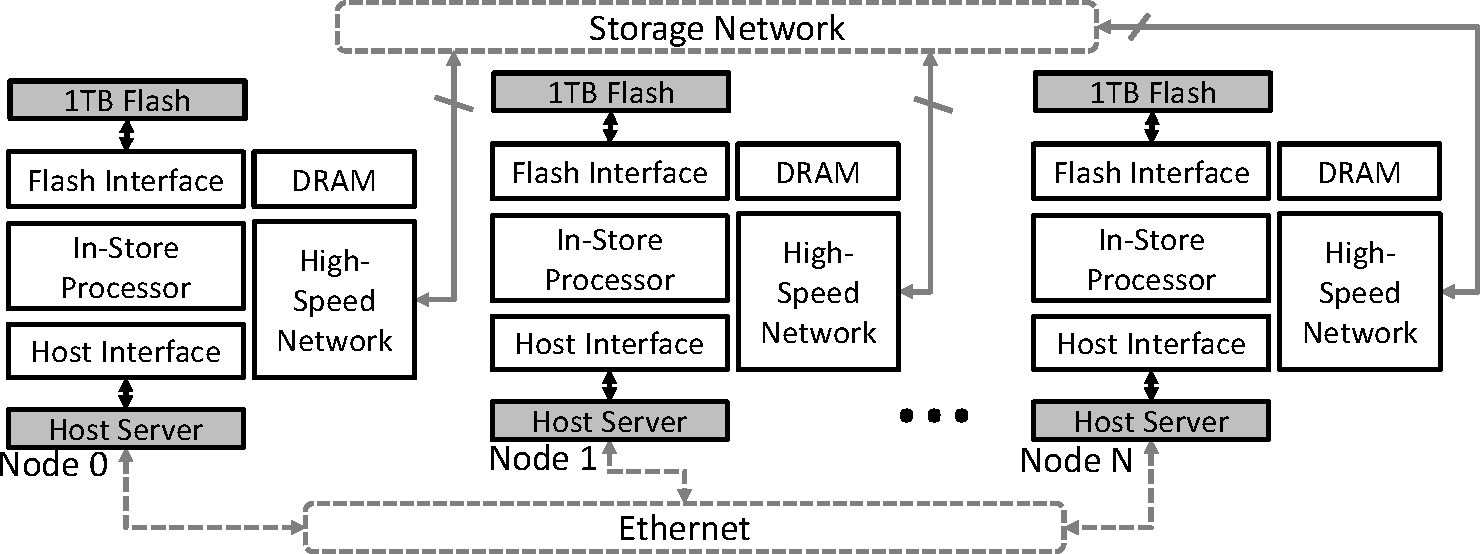
\includegraphics[width=0.8\paperwidth]{figures/architecture-crop.pdf}
	\caption{FlashBoost Architecture}
	\label{fig:architecture}
	\end{center}
\end{figure*}


\section{Motivation}

Computation/Storage coupling \(computation near data\), for MapReduce, etc



\section{Related Work}
\label{sec:related}

%Modern analytics systems are usually built as a cluster of homogeneous machines
%networked using a fast interconnect. In such a configuration, the system can
%perform at its full potential if the dataset can fit in its collective DRAM.

In Big Data scale workloads, building a cluster with enough DRAM capacity to
accommodate the entire dataset can be very desirable but expensive. An example
of such a system is RAMCloud, which is a DRAM-based storage for large-scale
datacenter applications~\cite{ramcloud, rumble_log_dram}.  RAMCloud provides more than 64TBs of DRAM
storage distributed across over 1000 servers networked over high-speed
interconnect. Although RAMCloud provides 100 to 1000 times better performance
than disk-based systems of similar scale, its high energy consumption and high
price per GB limits its widespread use except for extremely performance and
latency sensitive workloads.

NAND-Flash-based SSD devices are gaining traction as a faster alternative to
disks, and close the performance gap between DRAM and persistent storage.
SSDs have the benefit of an order of magnitude cheaper price compared to DRAM,
and an order of magnitude faster performance compared to disk.
Many existing database and analytics softwares have been demonstrated to have
improved performance with SSDs~\cite{hadoopperf,ssdhadoop,ssddatabase}.
Several SSD-optimized analytics softwares, such as the SanDisk
Zetascale~\cite{zetascale} have demonstrated promising
performance while using SSD has the primary data storage.
Many commercial SSD devices have adopted high-performance PCIe interface in
order to overcome the slower SATA bus interface designed for
disk~\cite{fusionio, violinmemory, intelnvme}. Attempts to
use flash as a persistent DRAM alternative by plugging it into a RAM slot
are being explored as well~\cite{diablotechnology}. 

SSD storage devices have been largely developed to be a faster drop-in
replacement for disk drives. This backwards compatibility helped them gain
widespread adoption.  However, this required additional software and hardware to
hide the difference in device characteristics~\cite{ssddesigntradeoff}.  Due to the high performance of
SSDs, even inefficiencies in the storage management software becomes
significant, and optimizing such software has been under active investigation.
Moneta~\cite{ucsd_moneta} modifies the operating system's storage management
components to reduce software overhead when accessing NVM storage devices.
Willow~\cite{ucsd_willow} provides an easy way to augment SSD controllers with
additional interface semantics that make better use of SSD characteristics, in
addition to a backwards compatible storage interface.  Attempts to remove the
translation layers and let the databse make high-level decisions~\cite{noftl}
have shown to be beneficial. 

Another important attempt to accelerate SSD storage performance is in-storage
processing, where some data analytics is offloaded to embedded processors inside
SSDs. These processors have extremely low-latency access to storage, and helped
overcome the limitations of the storage interface bus. The idea of in-storage
processing itself is not new. The idea of intelligent disks (IDISK) connected to
each other using serial networks have been proposed in 1998~\cite{idisk}, and
adding processor to disk heads to do simple filters have been suggested as early
as in the 1970s~\cite{searchprocessor,RAP,dbc}. However, performance improvements of such special
purpose hardware did not justify their price at the time. This idea is seeing
new light with advancement of fast flash devices. This idea is seeing new light
with the advancement of fast flash technology. Devices such as Smart
SSDS~\cite{smartssdquery,smartssdcost,ucsd_willow} and Programmable
SSDs~\cite{xsd} have been investigated and showed promising results. Because of
the limited performance of embedded processors on such power-constrained
devices, embedding reconfigurable hardware on storage devices are being
investigated as well. Ibex~\cite{ibex} is a MySQL accelerator platform where a
SATA SSD is coupled with an FPGA. Relational operators such as selection and
group-by are performed on the FPGA whenever possible, otherwise they are
forwarded to software. On the other end of the spectrum, systems such as
XSD~\cite{xsd} embeds a GPU into a SSD controller, and demonstrates high
performance accelerating MapReduce.

Due to their high performance, SSDs also effect the network requirements.  The
latency to access disk over Ethernet was dominated by the disk seek latency.
However, in a SSD-based cluster the storage access latency could even be lower
than network access. These concerns are being addressed by faster network
fabrics such as 10GbE and Infiniband~\cite{infiniband}, and by low-overhead
software protocols such as RDMA~\cite{rdmampi, rdmahdfs, homrmapreduce, rdmahpc,
rdmampi, hadoopinfiniband} or user-level TCP stacks that bypass the operating
system~\cite{usertcp,userlevelprotocol}. QuickSAN~\cite{ucsd_quicksan} is an
attempt to remove a layer of software overhead by augmenting the storage device
with a low-latency NIC, so that remote storage access does not need to go
through a separate network software stack.


Building specialized hardware for databases have been extensively studied and
productized. Companies such as Oracle~\cite{exadata} and
IBM/Netezza~\cite{netezza} have used FPGAs to offload database queries.
FPGAs have been used to accelerate operations such as hash index
lookups~\cite{walkers}. Domain-specific processors for database queries are
being developed~\cite{databasefpga, hybridsql}, including Q100~\cite{q100} and LINQits~\cite{linqits}.
Q100 is a data-flow style processor with an instruction set architecture that
supported SQL queries. LINQits mapped a query language called LINQ to a set of
accelerated hardware templates on a heterogeneous SoC (FPGA + ARM). Both designs
exhibited order of magnitude performance gains at lower power, affirming that
specialized hardware for data processing is very advantageous.
%However, in both cases, experiments were
%conducted with data that is on-chip or in DRAM.
Some database accelerators benefit from being on the datapath of normal data
movement. Accelerators have been place in-path to perform low-latency operations
at wire speed~\cite{fpgastreamquery}, or to collect information such as
histogram tables~\cite{histogramssideeffect}.

\begin{figure*}[t!]
\centering
\vspace{0pt}
\begin{minipage}[c]{.4\paperwidth}
\begin{center}
	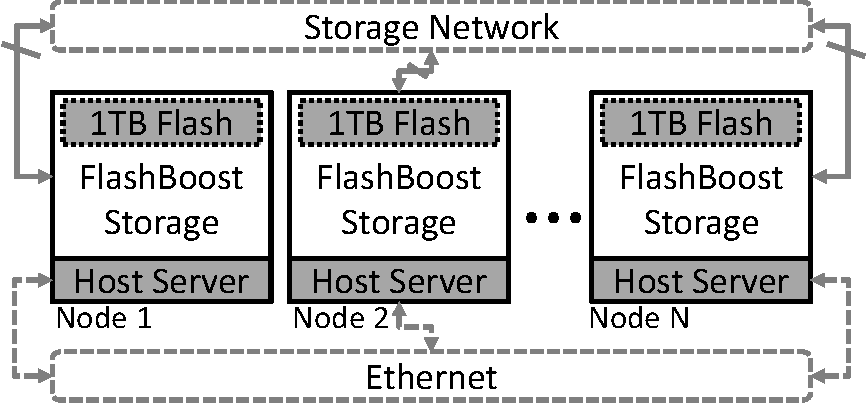
\includegraphics[width=\textwidth]{figures/architecture_small-crop.pdf}
	\caption{FlashBoost Overall Architecture}
	\label{fig:architecture}
\end{center}
\end{minipage}\hfill
\vspace{0pt}
\begin{minipage}[c]{.4\paperwidth}
\begin{center}
	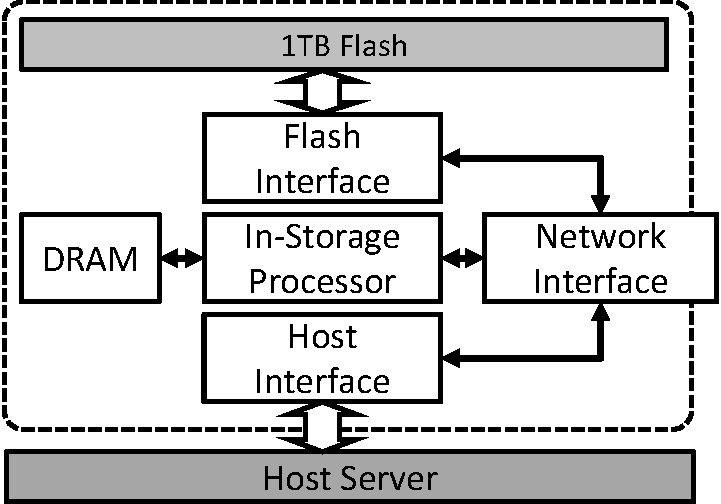
\includegraphics[width=0.7\textwidth]{figures/architecture_node-crop.pdf}
	\caption{FlashBoost Node Architecture}
	\label{fig:architecture_node}
\end{center}
\end{minipage}
\end{figure*}



Incorporating reconfigurable hardware accelerators into large datacenters are
being actively investigates as well. Microsoft recently has built and
demonstrated the power/performance benefits of a FPGA-based system called
Catapult~\cite{msr_catapult}.  Catapult uses a large number of homogeneous
servers each augmented with an FPGA.  The FPGAs form a network among themselves
via high-speed serial links so that large jobs can be mapped to groups of FPGAs.
Catapult was demonstrated to deliver much faster performance while consuming
less power, compared to a normal ram cloud cluster. FlashBoost has similar
goals in terms of reconfigurable hardware acceleration, but it uses flash
devices to accelerate lower cost systems that do not have enough collective DRAM
to host the entire dataset.

FlashBoost incorporates ideas such as in-storage processing and integrated
networks to construct a high-performance flash-based analytics appliance.
Previous work such as BlueDBM~\cite{bluedbm} have included similar features, but
FlashBoost differs in the sense that it has enough capacity to explore
real-world Big Data applications.

\section{System Architecture}
\label{sec:architecture}


The FlashBoost architecture is a homogeneous cluster of host servers coupled
with a FlashBoost storage device. Each FlashBoost storage device is plugged into
the host server via a PCIe link, and it consists of flash storage, an in-storage
processing engine, 8 high-speed network interfaces and on-board DRAM. The host
servers are networked together using Ethernet or other general-purpose
networking fabric. The host server can access the FlashBoost storage device via
a host interface implemented over PCIe. It can either directly communicate with
the flash interface, to treat is as a raw storage device, or with the in-store
processor to perform computation on the data.

The in-store processing engine has access to four major services: The flash
interface, network interface, host interface and the on-storage DRAM buffer.
Figure~\ref{fig:architecture_node} shows the four services available to the
in-storage processor. In the following sections we describe the flash interface,
network interface and host interface in order. We omit the DRAM buffer because
its design is very generic.

\subsection{Flash Interface}

Flash devices or SSDs achieve high bandwidth by grouping multiple flash chips
into several channels, all of which can operate in parallel. Because NAND flash
has limited program/erase cycles and frequent errors, complex flash management
algorithms are required to guarantee reliability. These include wear leveling,
garbage collection, bit error correction and bad block management. These
functions are typically handled by multiple ARM-based cores in the SSD
controller. The host side interface of an SSD is typically SATA or PCIe, using
AHCI or NVMe protocols to communicate with host. SSDs are viewed
as a typical block device to the host operating system, and its internal
architecture and management algorithms are completely hidden. 

However, this additional layer of management has shown to be duplicated with
file system functionalities and adds significant latency~\cite{redo}.
Furthermore, in a distributed storage environment, such as FlashBoost,
independent flash devices do not have a holistic view of the system and thus
cannot efficiently manage flash. Finally, in-store processors that we have
introduced in FlashBoost would also incur performance penalties if passing
through this extra layer. 

Thus in FlashBoost, we chose to shift flash management
away from the device and into file system/block device driver (discussed in
Section~\ref{sec:software}). Our flash controller exposes a low-level, thin,
fast and bit-error corrected hardware interface to raw NAND flash chips, buses,
blocks and pages. This has the benefit of (i) cutting down on access latency
from the network and in-store processors; (ii) exposing all degrees of
parallelism of the device and (iii) allowing higher level system stacks (file
system, database storage engine) to more intelligently manage data. 

To access the flash, the user first issues a flash command
with the operation, the address and a unique tag.
For writes, the user then awaits for a write data request from
the controller scheduler, which tells the user that the flash controller is
ready to receive the data for that write. The user will send the write data
corresponding to that request in 128-bit bursts. The controller returns an
acknowledgement once write is finished. 
For read operations, after a command is issued,
data will return in 128-bit bursts along with the command tag that the
burst corresponds to. We emphasize that for maximum performance, the
controller may send these data bursts \emph{out of order} with respect to
the issued request and \emph{interleaved} with other read requests.
Thus completion buffers may be required on the user side to maintain FIFO
characteristics. Furthermore,
we note that to saturate the bandwidth of the flash device, multiple
commands must be in-flight at the same time, since flash operations
can have latencies of 50 $\mu s$ or more. 

%Access to flash storage is provided by the flash controller via a fast,
%low-level and error-free interface with minimal overhead. This interface exposes
%the internal memory organization of the flash device, namely the buses/channels,
%chips, blocks and pages.  The interface is designed to stream data in and out of
%the flash chips as fast as possible without concern for flash management. Flash
%management functionalities such as garbage collection, bad block management and
%wear-leveling are handled by the flash-aware file system described int
%Section~\ref{sec:software}, or implemented inside the in-store processor itself.
%The key advantage of such a low-level interface is that the in-store processors
%have direct access to data with minimal overhead.

\begin{figure}[h]
	\begin{center}
	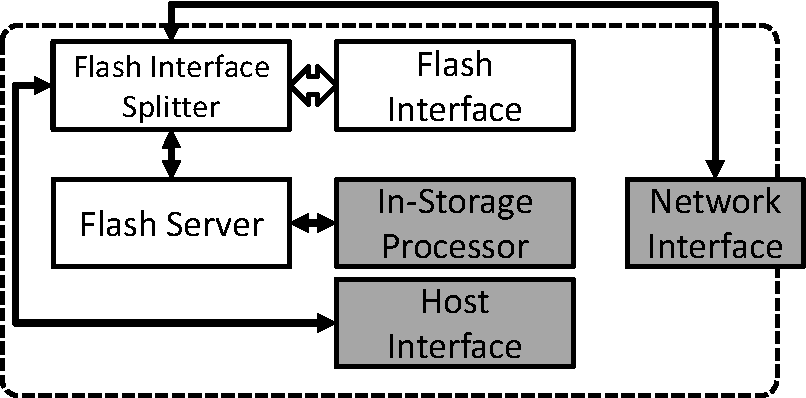
\includegraphics[scale=0.4]{figures/architecture_flash-crop.pdf}
	\caption{Flash Interface}
	\label{fig:flashinterface}
	\end{center}
\end{figure}

\subsubsection{Multiple Access Agents}

Multiple hardware endpoints in FlashBoost may need shared access to this
flash controller interface. For example, a particular controller may
be accessed by local in-store processors, local host software over PCIe
DMA, or remote in-store processors over the network. Thus we implemented a
Flash Interface Splitter with tag renaming to manage multiple users
(Figure~\ref{fig:flashinterface}). In addition, 
to ease development of hardware in-store processors,
we also provide an optional Flash Server module as part of FlashBoost. This server
converts the out-of-order and interleaved flash interface into
multiple simple in-order request/response interfaces
using page buffers. It also contains an Address Translation Unit that 
maps file handles to incoming streams of physical addresses from the host. The in-store processor
simply makes a request with the file handle, offset and length, and the Flash Server will perform
the flash operation at the corresponding physical location. The software
support for this function is discussed in Section~\ref{sec:software}). The Flash
Server's width, command queue depth and number of interfaces is adjustable 
based on the application.

\subsection{Integrated Storage Network}

\begin{figure}[t]
	\begin{center}
	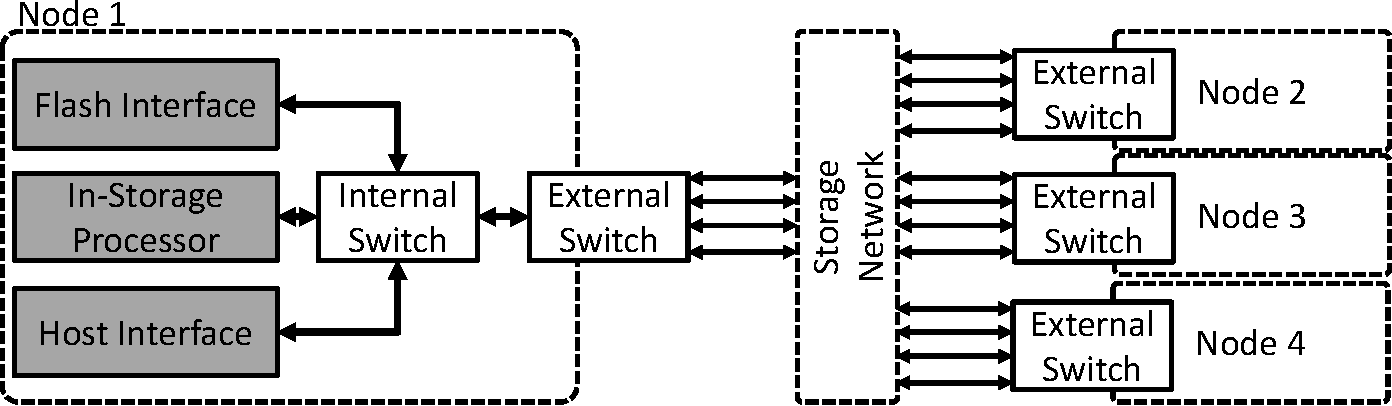
\includegraphics[width=0.5\textwidth]{figures/network-architecture-crop.pdf}
	\caption{Network Architecture}
	\label{fig:networkinterface}
	\end{center}
\end{figure}


FlashBoost provides a low-latency high-bandwidth network infrastructure across
all FlashBoost storage devices in the cluster, while maintaining a simple design
with low resource usage. FlashBoost storage devices form a separate network
among themselves via high-performance serial links.  The FlashBoost network is a
packet-switched mesh network, in which each storage device has multiple network
ports and is capable of routing packets across the network without requiring a
separate switch or router.  In addition to routing, the storage network supports functionality such as
flow control and virtual channels while maintaining high performance and
extremely low latency.  For data traffic between the storage devices, the
integrated network ports removes the overhead of going to the host software to
access a separate network interface.

Figure~\ref{fig:networkinterface} shows the network architecture. Switching is
done at two levels, the internal switch and the external switch.  The internal
switch routes packets between local components.  The external switch accesses
multiple physical network ports, and is responsible for relaying data from a
port to another port in order to relay a packet to its next hop. It is also
responsible for relaying inbound packets to the internal
switch, and relaying outbound packets from the internal switch to a correct
physical port. 

Due to the multiple ports on the storage nodes, the FlashBoost network is very
flexible and can be configured to implement various topologies, as long as no
one node requires more connections than the number of ports on it.
Figure~\ref{fig:topologies} shows some example topologies. To implement a
different topology the physical cables between each node has to be re-wired, but
the routing across a topology can be configured dynamically by the software.

%Components that want to use the network choose one or more \emph{Logical
%Endpoints}, which provide virtual channel semantics, to access the network in a
%virtualized manner.

\begin{figure}[t!]
	\centering
	\subfloat[Distributed Star]
		{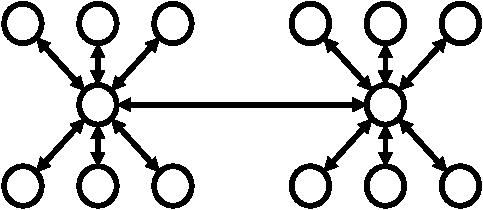
\includegraphics[scale=0.35]{figures/topology_dist_star-crop.pdf}}
		\hfill
	\subfloat[Mesh]
		{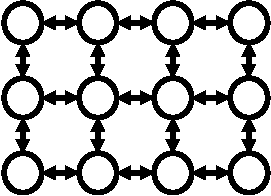
\includegraphics[scale=0.35]{figures/topology_mesh-crop.pdf}}
		\hfill
	\subfloat[Fat Tree]
		{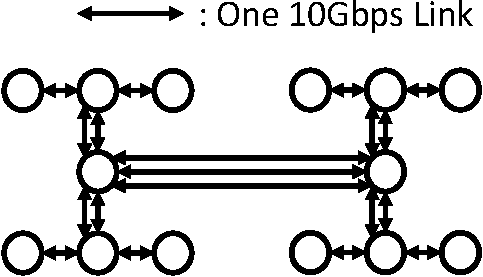
\includegraphics[scale=0.35]{figures/topology_fat_tree-crop.pdf}}
	\caption{Any Network Topology Is Possible As Long As It Requires Less Than 8
	Network Ports Per Node}
	\label{fig:topologies}
\end{figure}


\subsubsection{Logical Endpoint}

The FlashBoost network infrastructure exposes virtual channel semantics to the
users of the network by providing it with multiple \emph{logical endpoints}.  The
number of endpoints are determined at design time by setting a parameter, and
all endpoints share the physical network.  Each endpoint is parameterized with a
unique index that does not need to be contiguous.  Each endpoint exposes two
interfaces, \texttt{send} and \texttt{receive}. An in-storage processor can send
data to a remote node by calling \texttt{send} with a pair of data and
destination node index, or receive data from remote nodes by calling
\texttt{receive}, which returns a pair of data and source node index. These
interfaces provide back pressure, so that each endpoint can be treated like a
FIFO interface across the whole cluster. Such intuitive characteristics of the
network ease development of in-storage processors.

\subsubsection{Link Layer}

The link layer manages physical connections between network ports in the storage
nodes. The most important aspect of the link layer is the simple token-based
flow control implementation. This provides back pressure across the link and
assures that no packet will drop if the data rate is higher than what the
network can manage, or if the data is not received from the destination node
quick enough.

\subsubsection{Routing Layer}

%The goals of the FlashBoost network infrastructure is to
%maintain high bandwidth and low latency, while maintaining a simple design for
%embedded implementation. This requirement
%prompted many design choices.

\begin{figure}[h]
	\begin{center}
	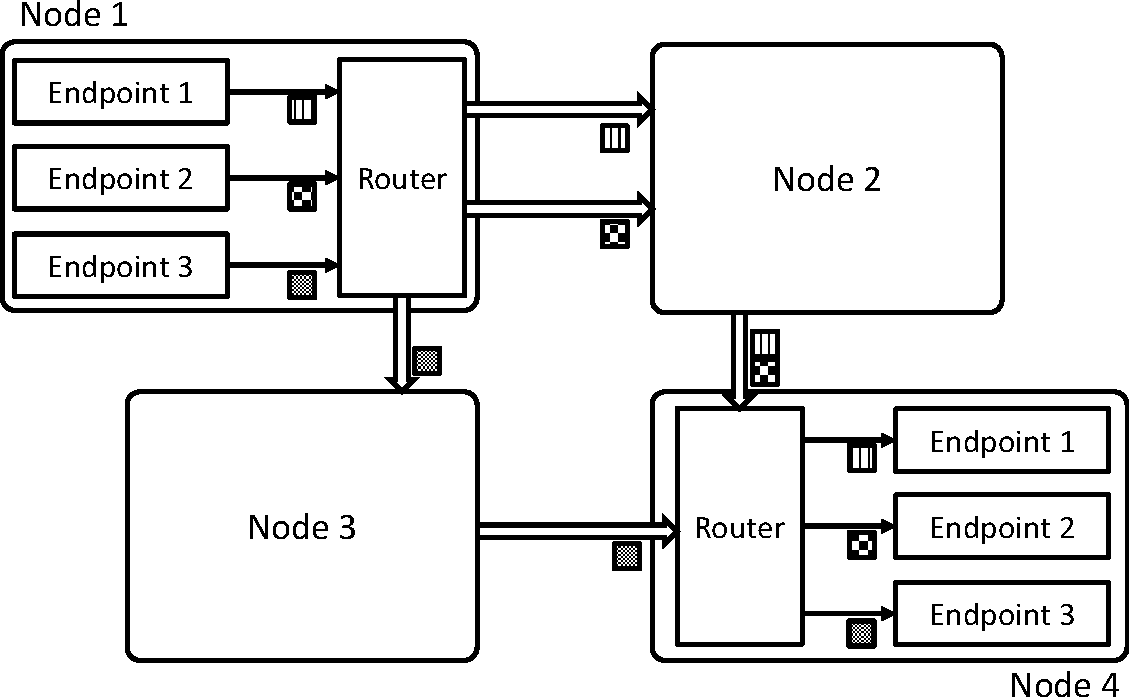
\includegraphics[width=0.4\textwidth]{figures/routing-crop.pdf}
	\caption{Routing Packets Across the Network}
	\label{fig:networkrouting}
	\end{center}
\end{figure}

In order to make maximum use of the bandwidth of the network infrastructure
while keeping resource usage to a minimal, the FlashBoost network implements
deterministic routing for each logical endpoint. This means that all packets
originating from the same logical endpoint that are directed to the same
destination node follow the same route across the network, while packets from a
different endpoint directed to the same destination node may follow a different
path. Figure~\ref{fig:networkrouting} shows packet routing in an example
network. The benefits of this approach is that packet traffic can be distributed
across multiple links, while maintaining the order of all packets from the same
endpoint. If packets from the same endpoint are allowed to take different paths,
it would require a completion buffer which may be expensive in an embedded
system.
For simplicity, the FlashBoost network does not implement a discovery protocol, and relies on a
network configuration file to populate the routing tables. 

In order to maintain extremely low network latency, each endpoint is given a
choice whether to use end-to-end flow control or not. If the developer is sure
that a particular virtual link will always drain on the receiving end, flow
end-to-end flow control can be omitted for that endpoint. However, if the
receiver fails to drain data for a long time, the link-level back pressure may
cause related parts of the network to block. On the other hand, an endpoint can
be configured to only send data when there is space on the destination endpoint,
which will assure safety but result in higher latency due to flow control
packets, and more memory usage for buffers.

\subsection{Host Interface}

The in-storage processing core can be accessed from the host server over either
a direct interface that supports RPC and DMA operations, or a file system
abstraction built on top of the direct interface. The file system interface is
described in detail in Section~\ref{sec:software}.

In order to parallelize requests and maintain high performance, the host
interface provides the software with 128 page buffers, each for reads and
writes. When writing a page, the software will request a free write buffer, copy
data to the write buffer, and send a write request over RPC with the
physical address of the destination flash page.
The buffer will be returned to the free queue when the
hardware has finished reading the data from the buffer. When reading a page, the
software will request a free read buffer, and send a read request over RPC with
the physical address of the source flash page. The software will receive an
interrupt with the buffer index when the hardware has finished writing to
software memory.

Using DMA to write data to the storage device is straightforward to parallelize,
but parallelizing reads is a bit more tricky due to the characteristics of flash
storage. When writing to storage, the DMA engine on the hardware will read data
from each buffer in order in a contiguous stream. So having enough requests in
the request queue is enough to make maximum use of the host-side link bandwidth.
However, data read from flash chips on multiple buses in parallel can arrive
interleaved at the DMA engine. Because the DMA engine needs to have enough
contiguous data for a DMA burst before issuing a DMA burst, some reordering may
be required at the DMA engine. This becomes even more tricky when the device is
using the integrated network to receive data from remote nodes, where they might
all be coming from different buses. To fix this issue, we provide dual-ported
buffer in hardware providing the semantics of a vector of FIFOs, so that data
for each request can be enqueued into its own FIFO until there is enough data
for a burst.
Figure~\ref{fig:hostinterface} describes the structure of the host interface for
flash reads.

\begin{figure}[t!]
	\centering
	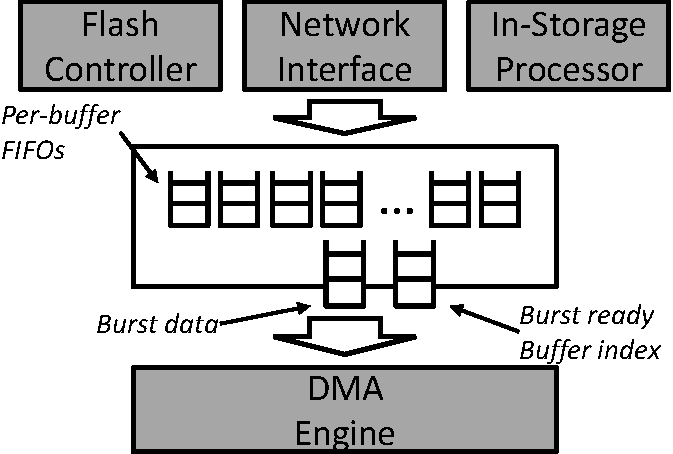
\includegraphics[width=0.3\textwidth]{figures/dmawrite-crop.pdf}
	\caption{Host-FPGA Interface Over PCIe}
	\label{fig:hostinterface}
\end{figure}

%TODO: \subsubsection{Storage Bridge to Host}


%%%% Comments!

\begin{comment}
The raw flash interface, in hardware, is defined below:

%[captionpos=b, caption={Flash Controller Interface}, label={lst:hwifc}]
\begin{lstlisting}
interface FlashIfc;       
  method sendCmd (FlashOp op, Bit#(4) bus,
                  Bit#(3) chip, Bit#(16) block, 
                  Bit#(8) page, Bit#(8) tag);        
  method writeWord (Bit#(128) data, Bit#(8) tag);
  method Tuple2#(Bit#(128), Bit#(8)) readWord (); 
  method Bit#(8) writeDataReq ();
  method Tuple2#(Bit#(8), StatusT) ackStatus ();
endinterface 
\end{lstlisting}
\end{comment}


\section{Hardware Implementation}
\label{sec:implementation}

We have built a 20-node FlashBoost cluster to explore the capabilities of the
architecture. Figure~\ref{fig:bluedbmcluster} shows the photo of our
implementation.

%\begin{figure}[ht]
%	\begin{center}
%	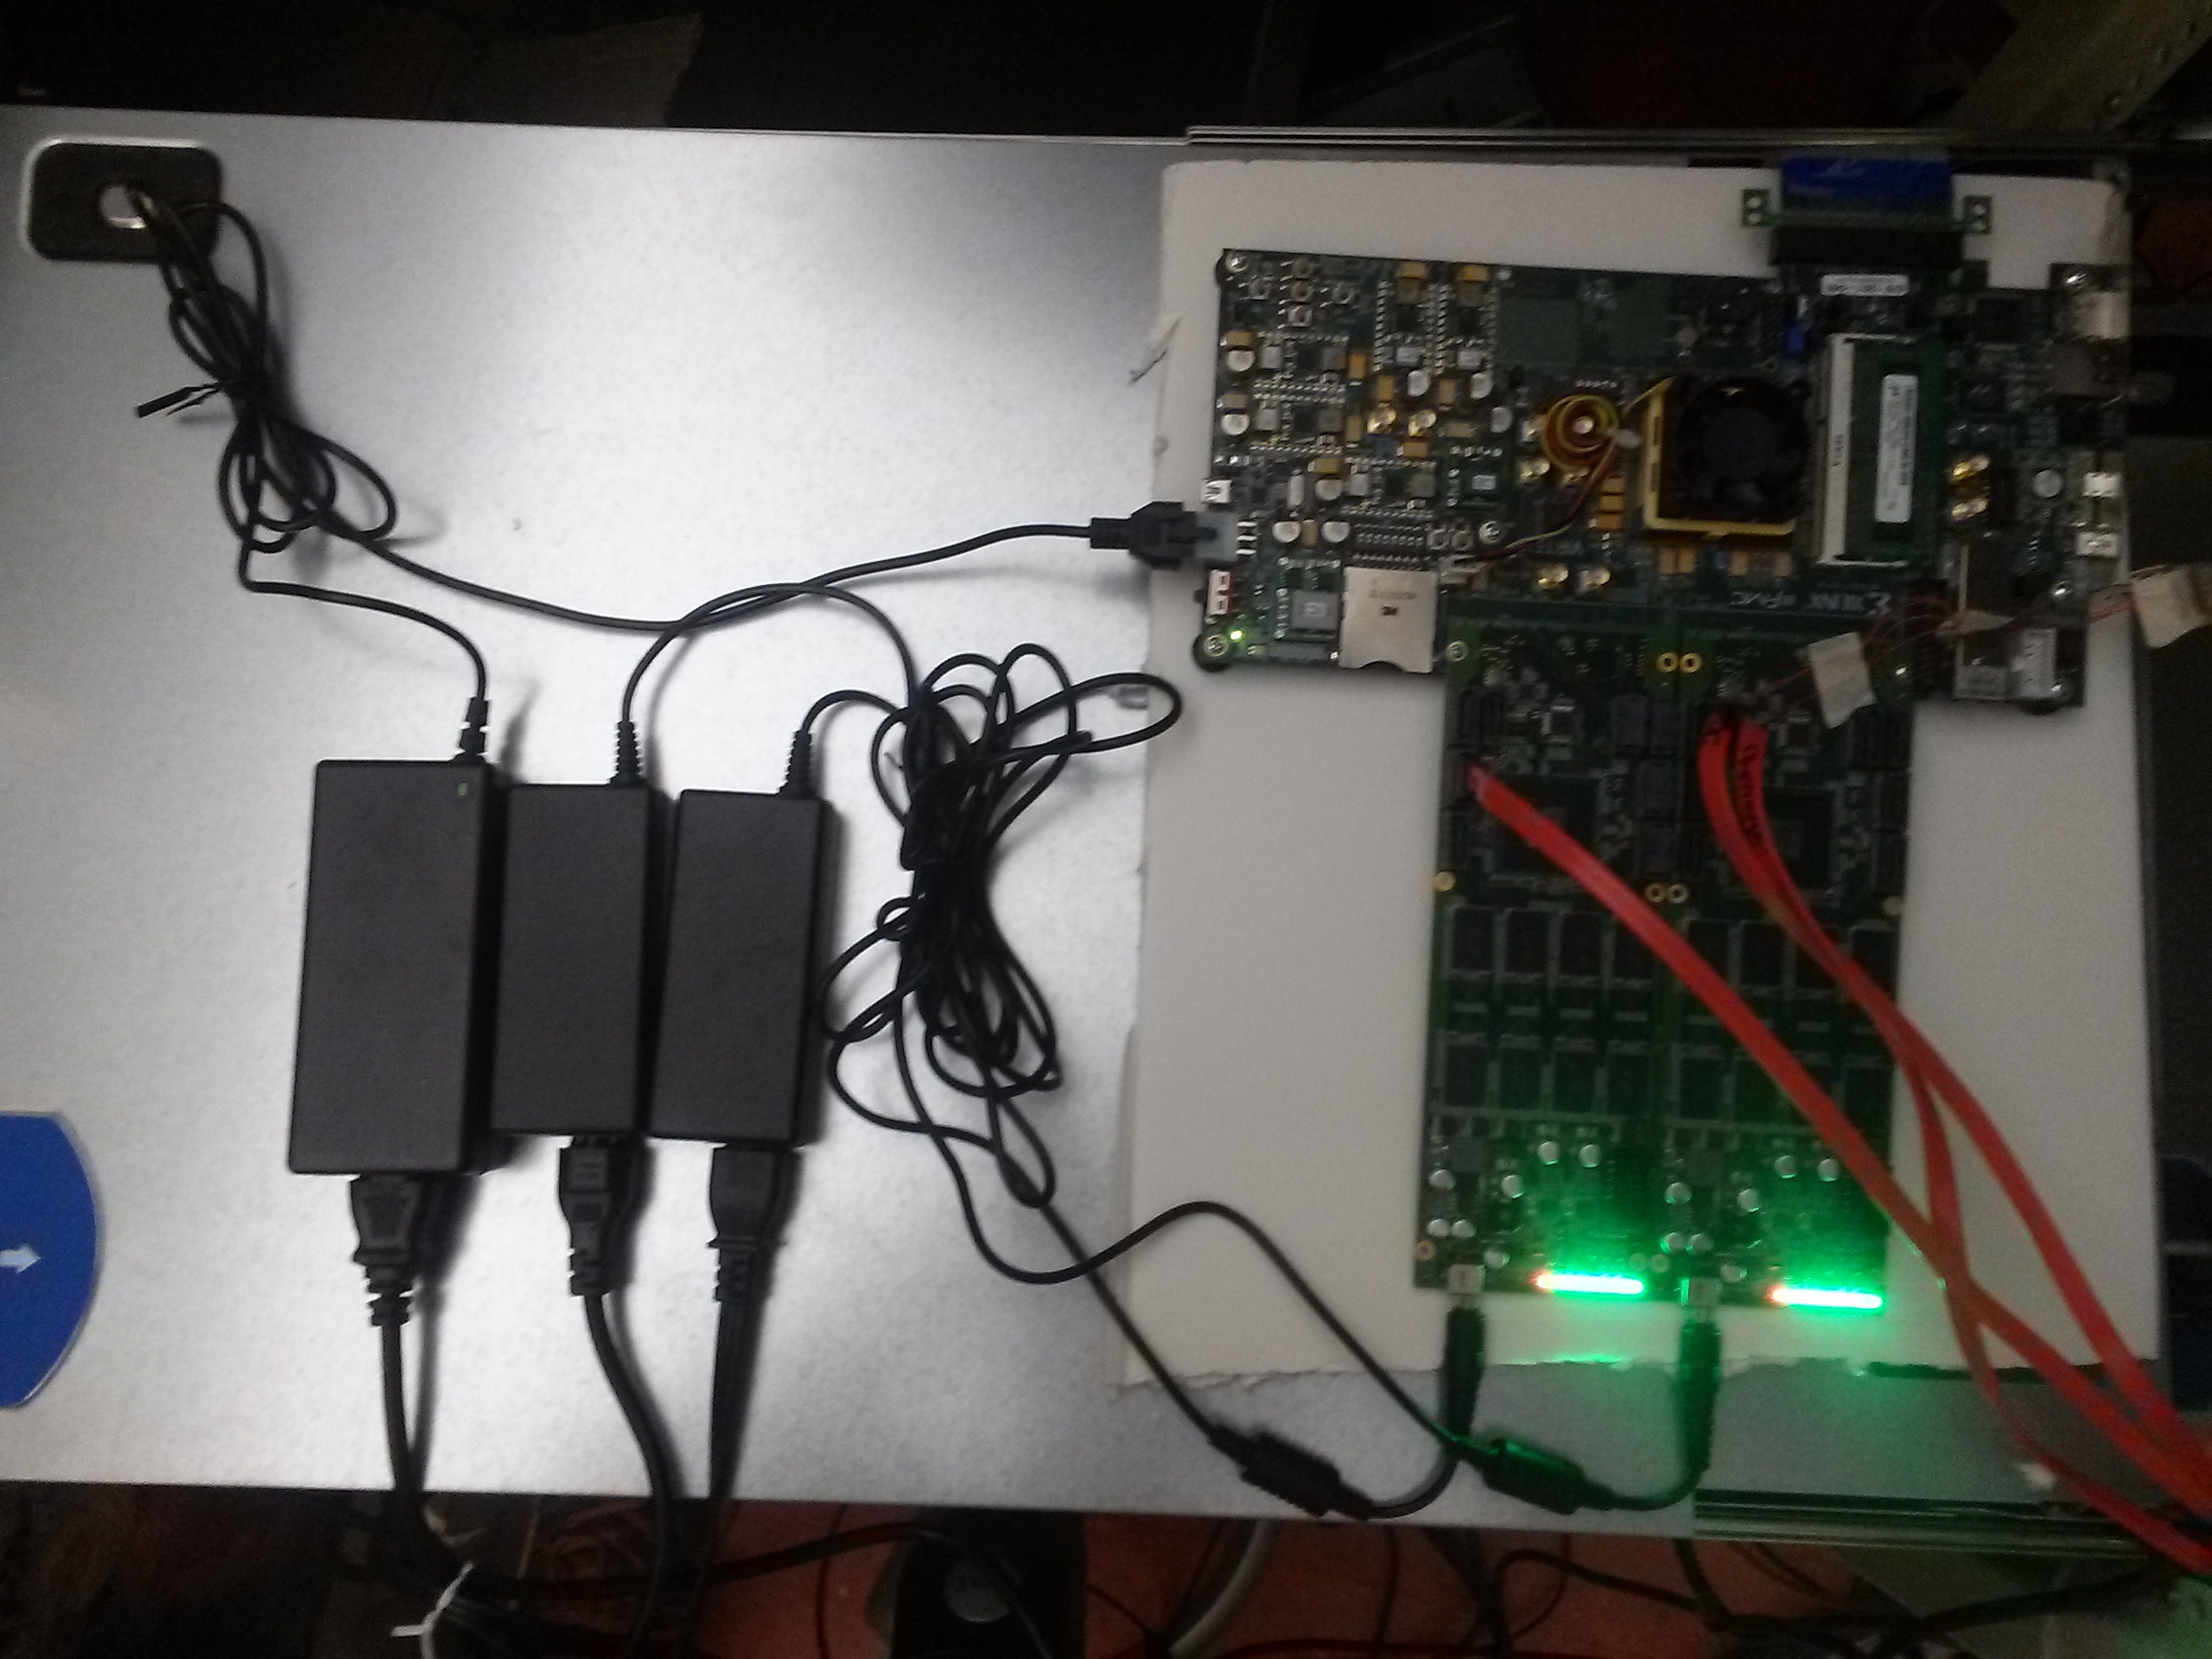
\includegraphics[width=0.3\paperwidth]{figures/rackserver.jpg}
%	%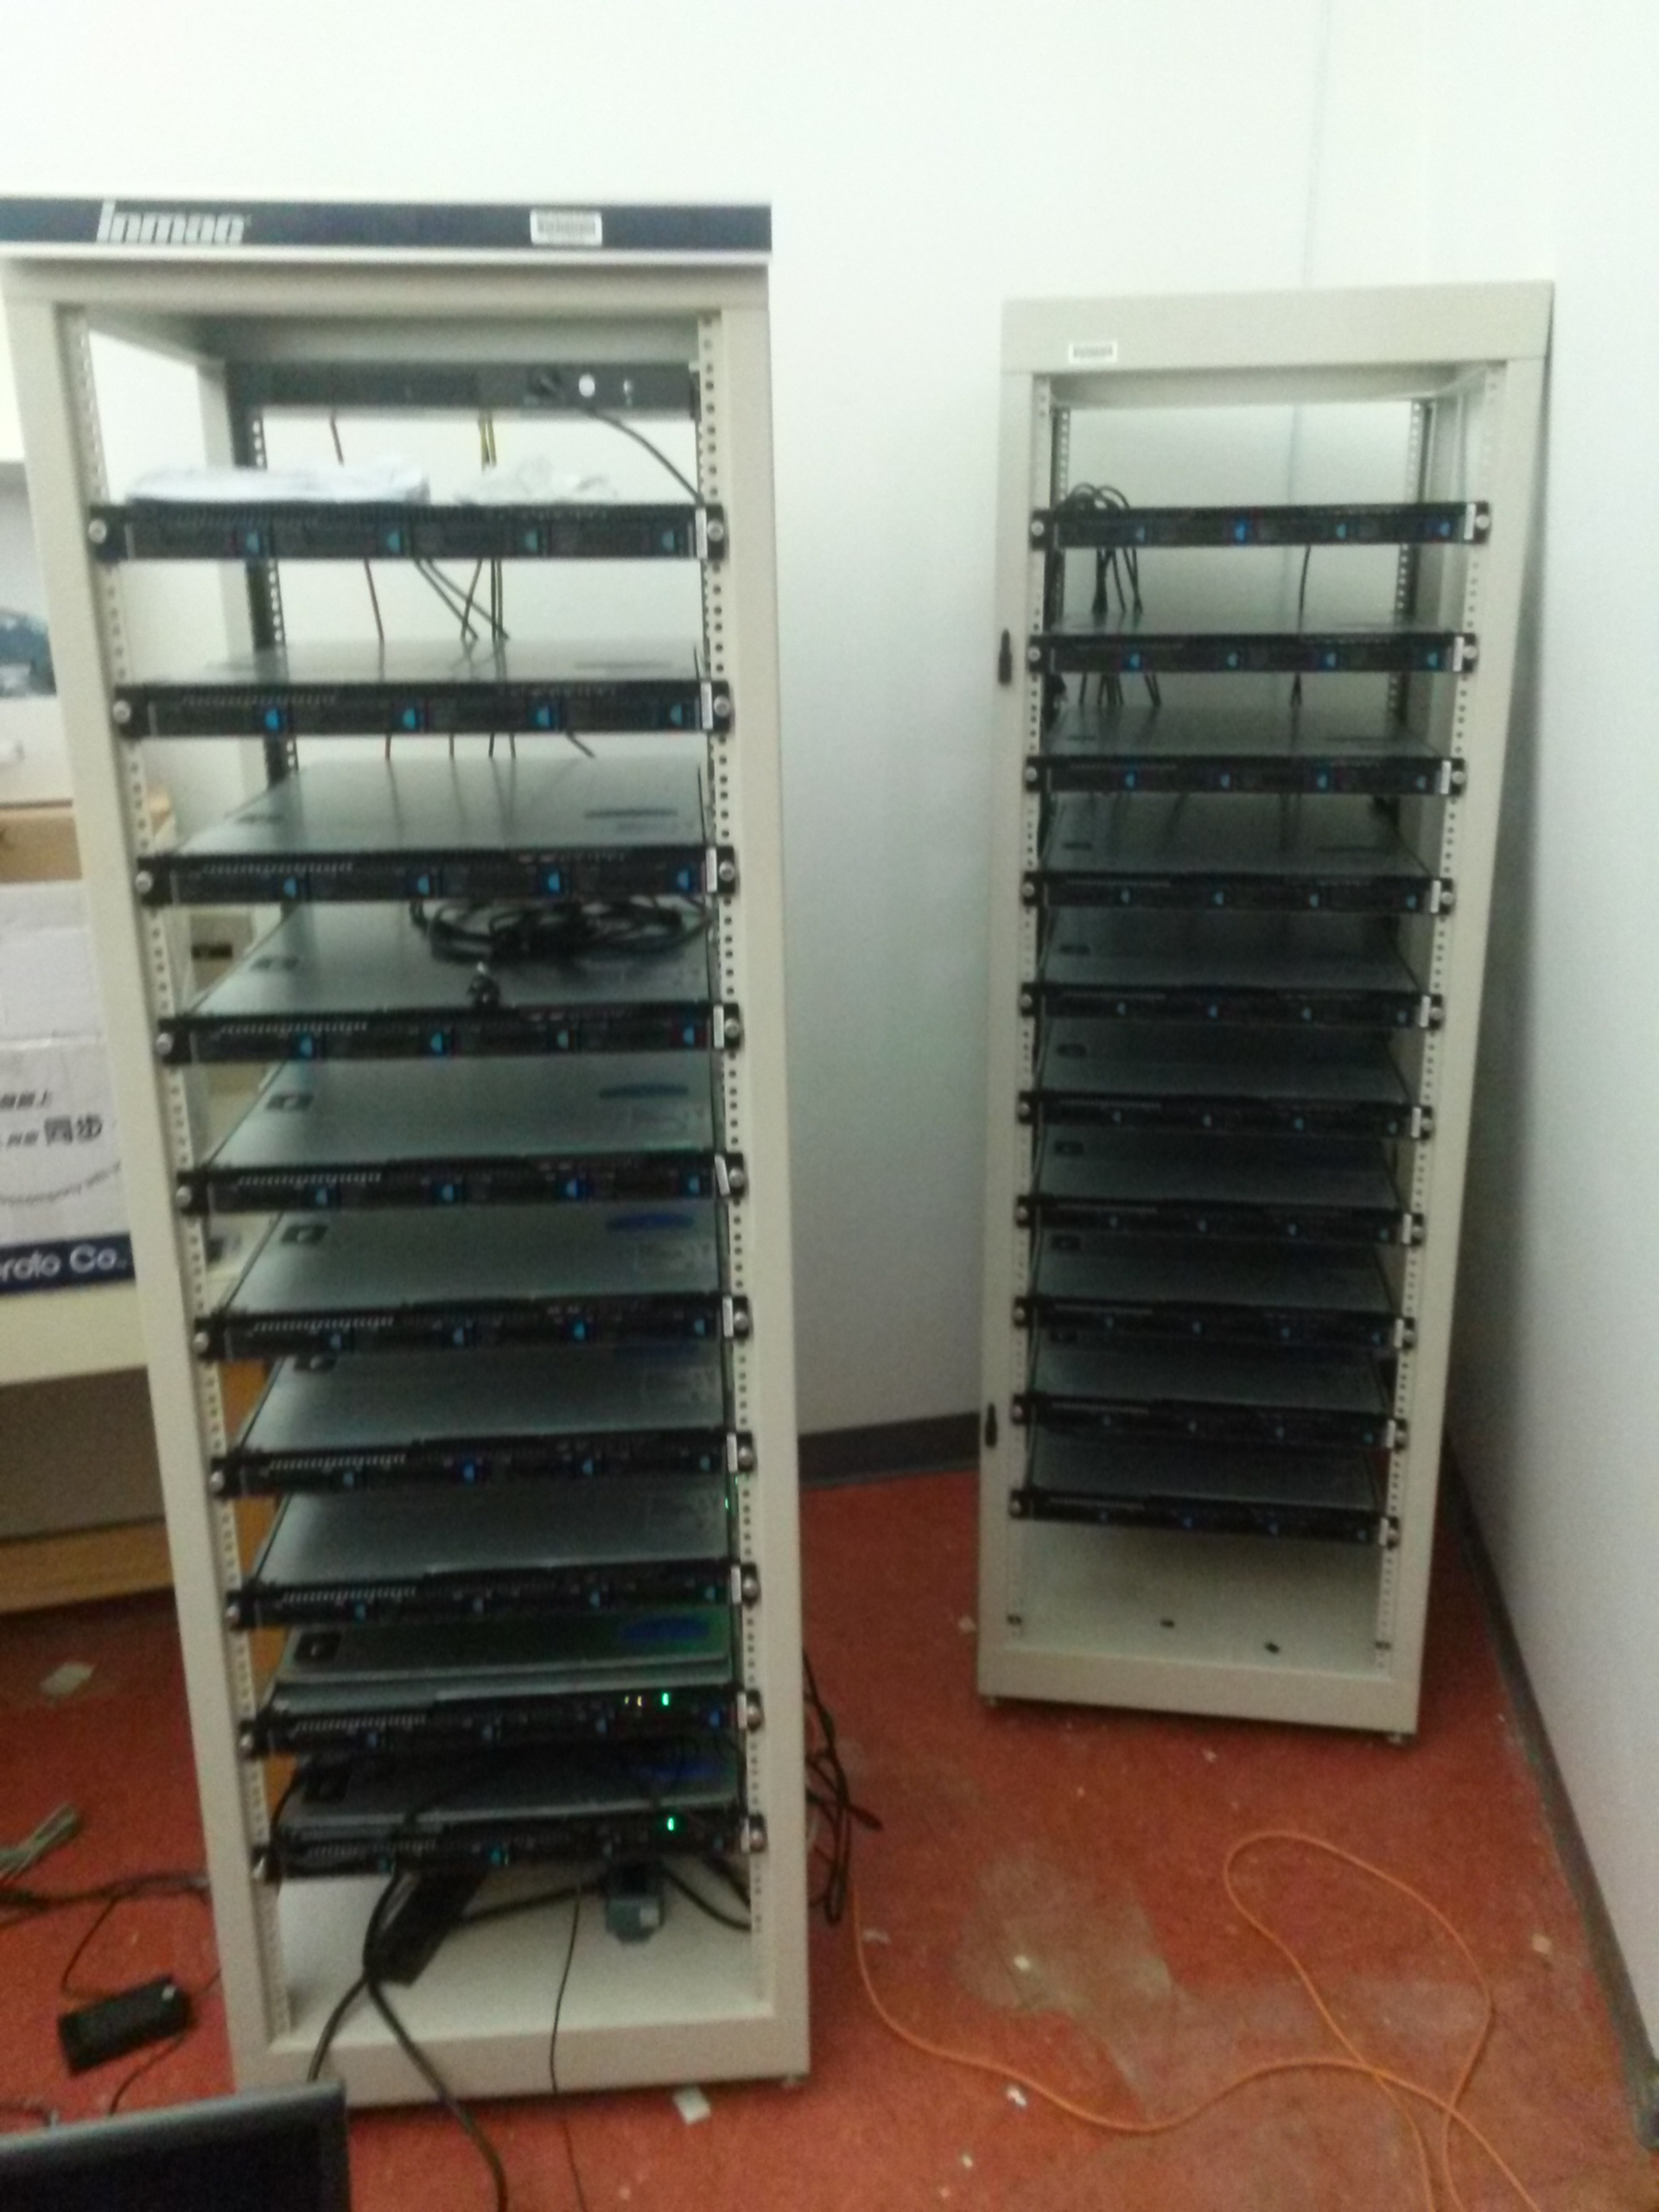
\includegraphics[width=0.3\paperwidth]{figures/rack.jpg}
%	\caption{A 20-node FlashBoost Cluster}
%	\label{fig:bluedbmcluster}
%	\end{center}
%\end{figure}

\begin{figure}[ht!]
	\begin{tabular}{cc}

	\multirow{2}{*}{
	\begin{minipage}[c]{.20\textwidth}
	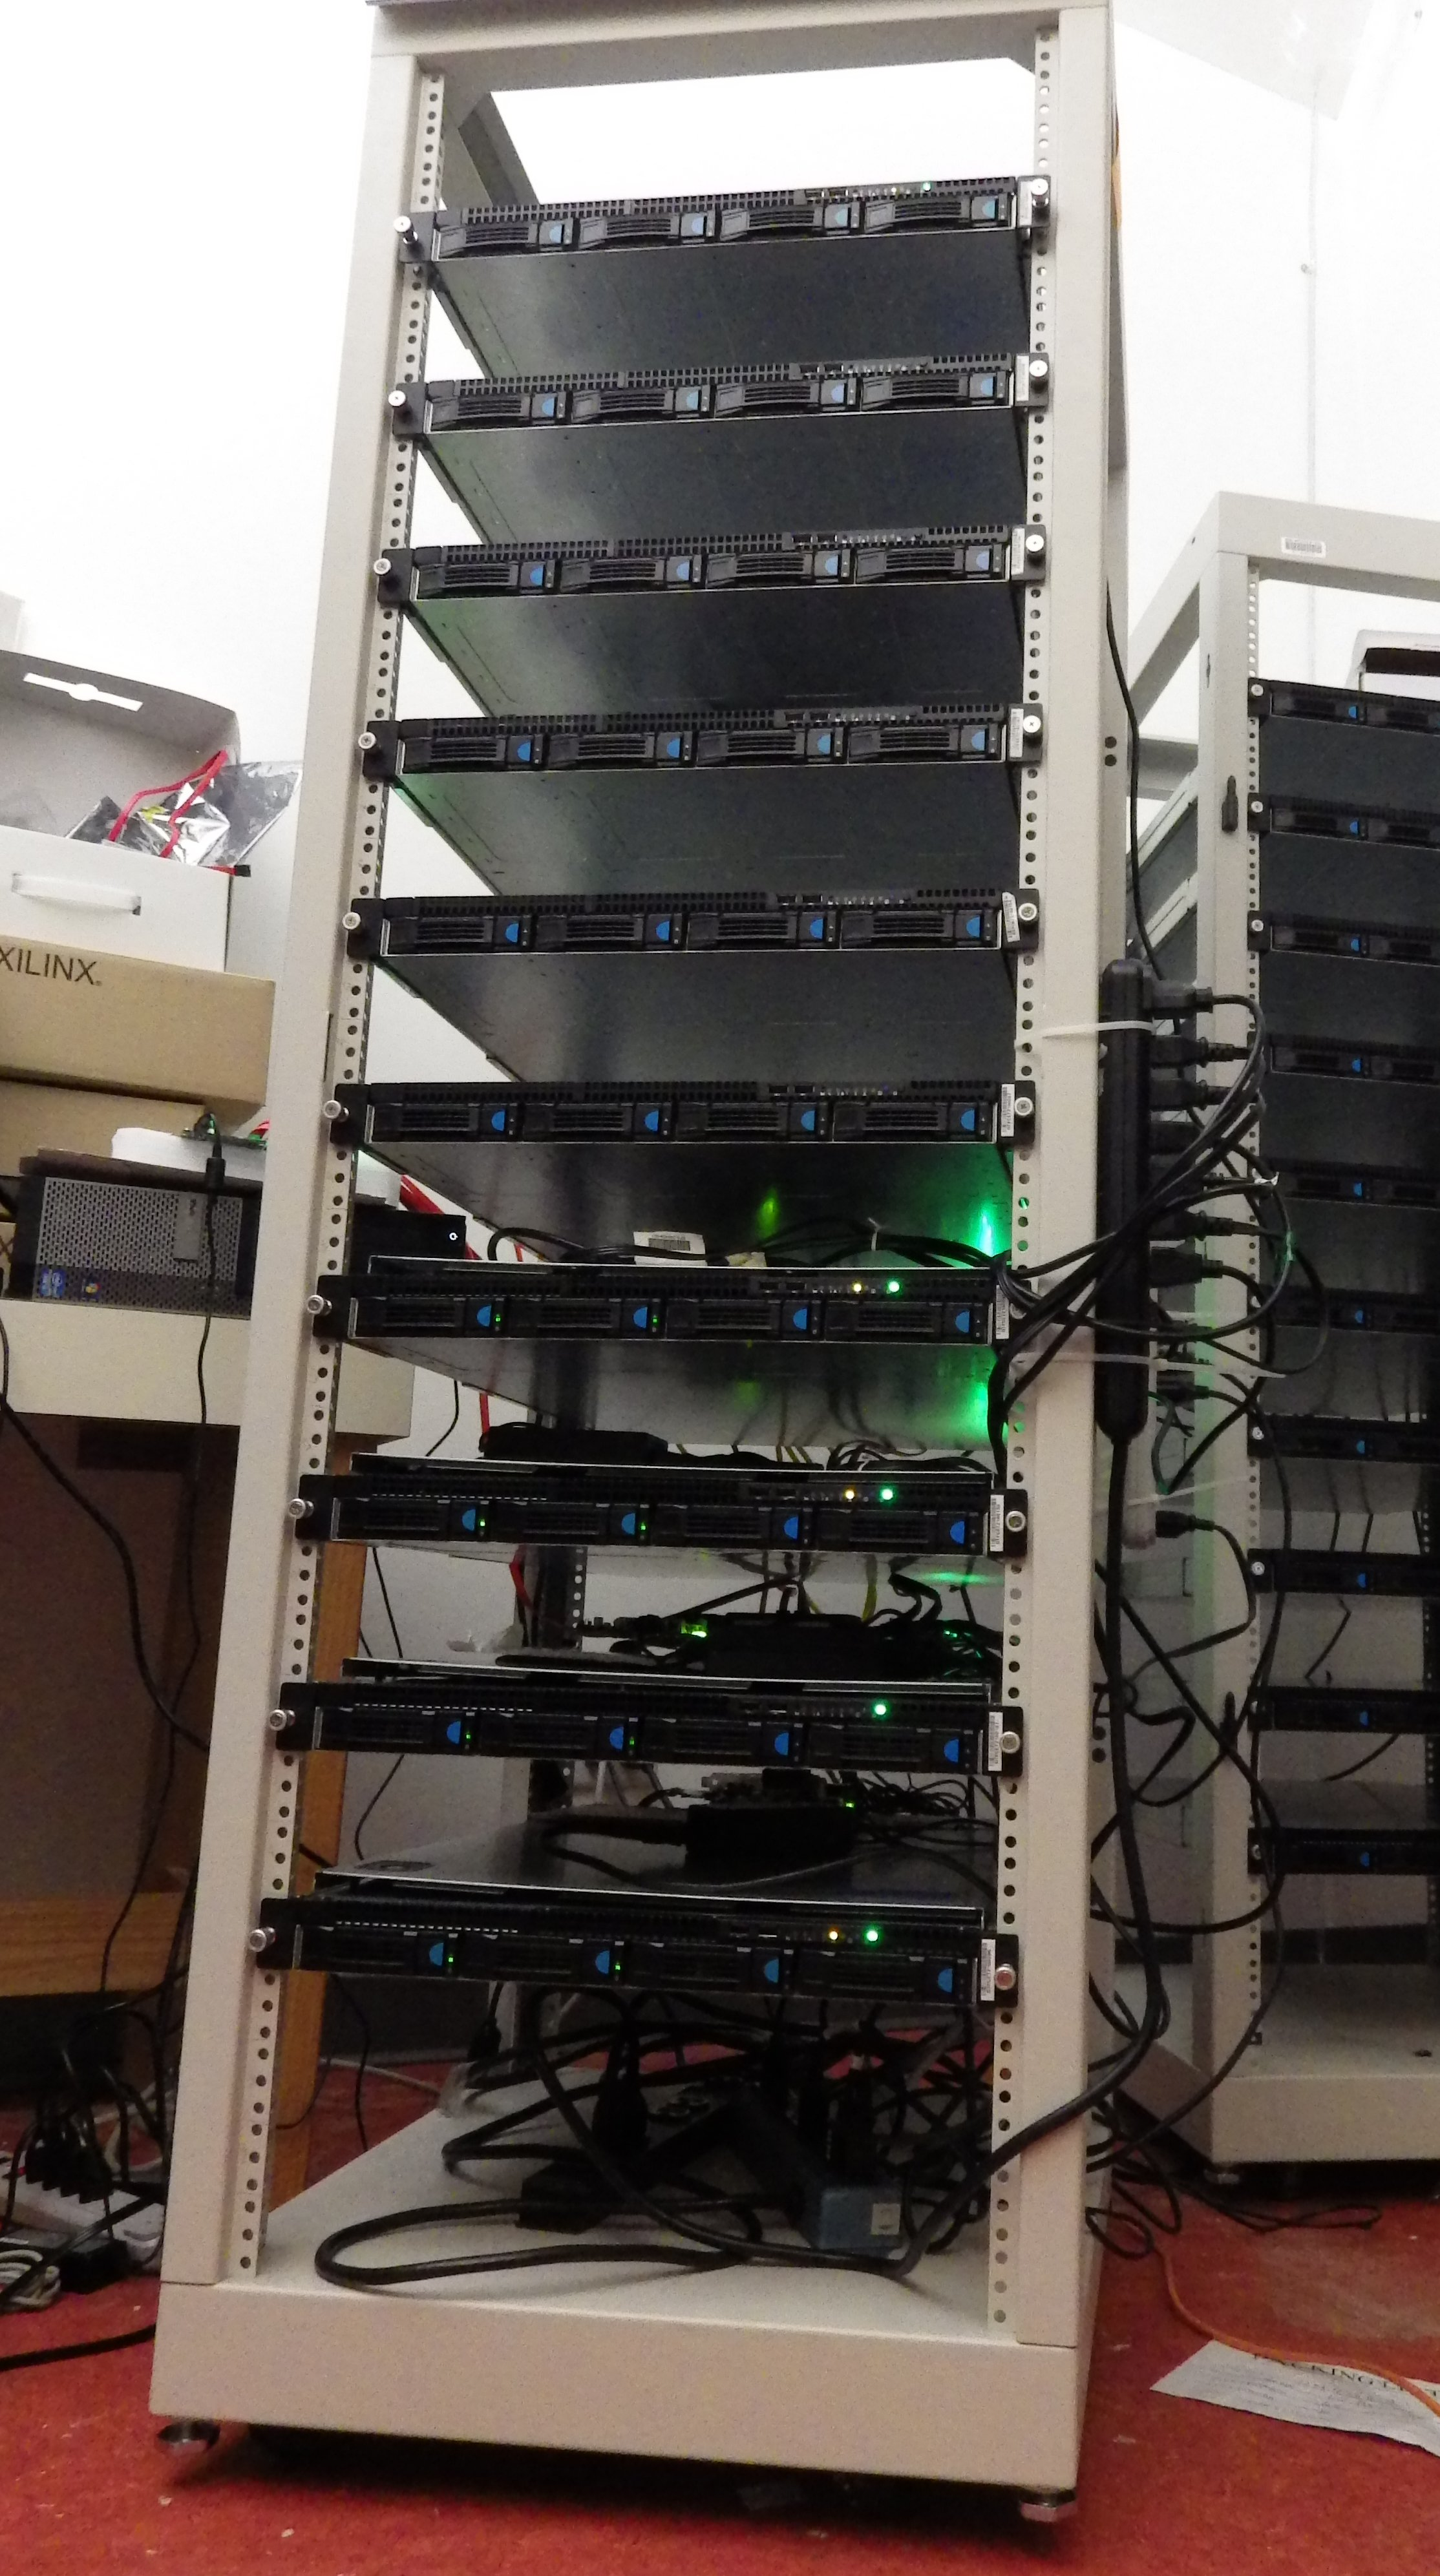
\includegraphics[width=\textwidth]{figures/rackserver2.jpg}
	\caption{One of the two 10-node FlashBoost Racks}
	\label{fig:bluedbmcluster}
	\end{minipage}
	}
	& 
	\begin{minipage}[c]{.20\textwidth}
	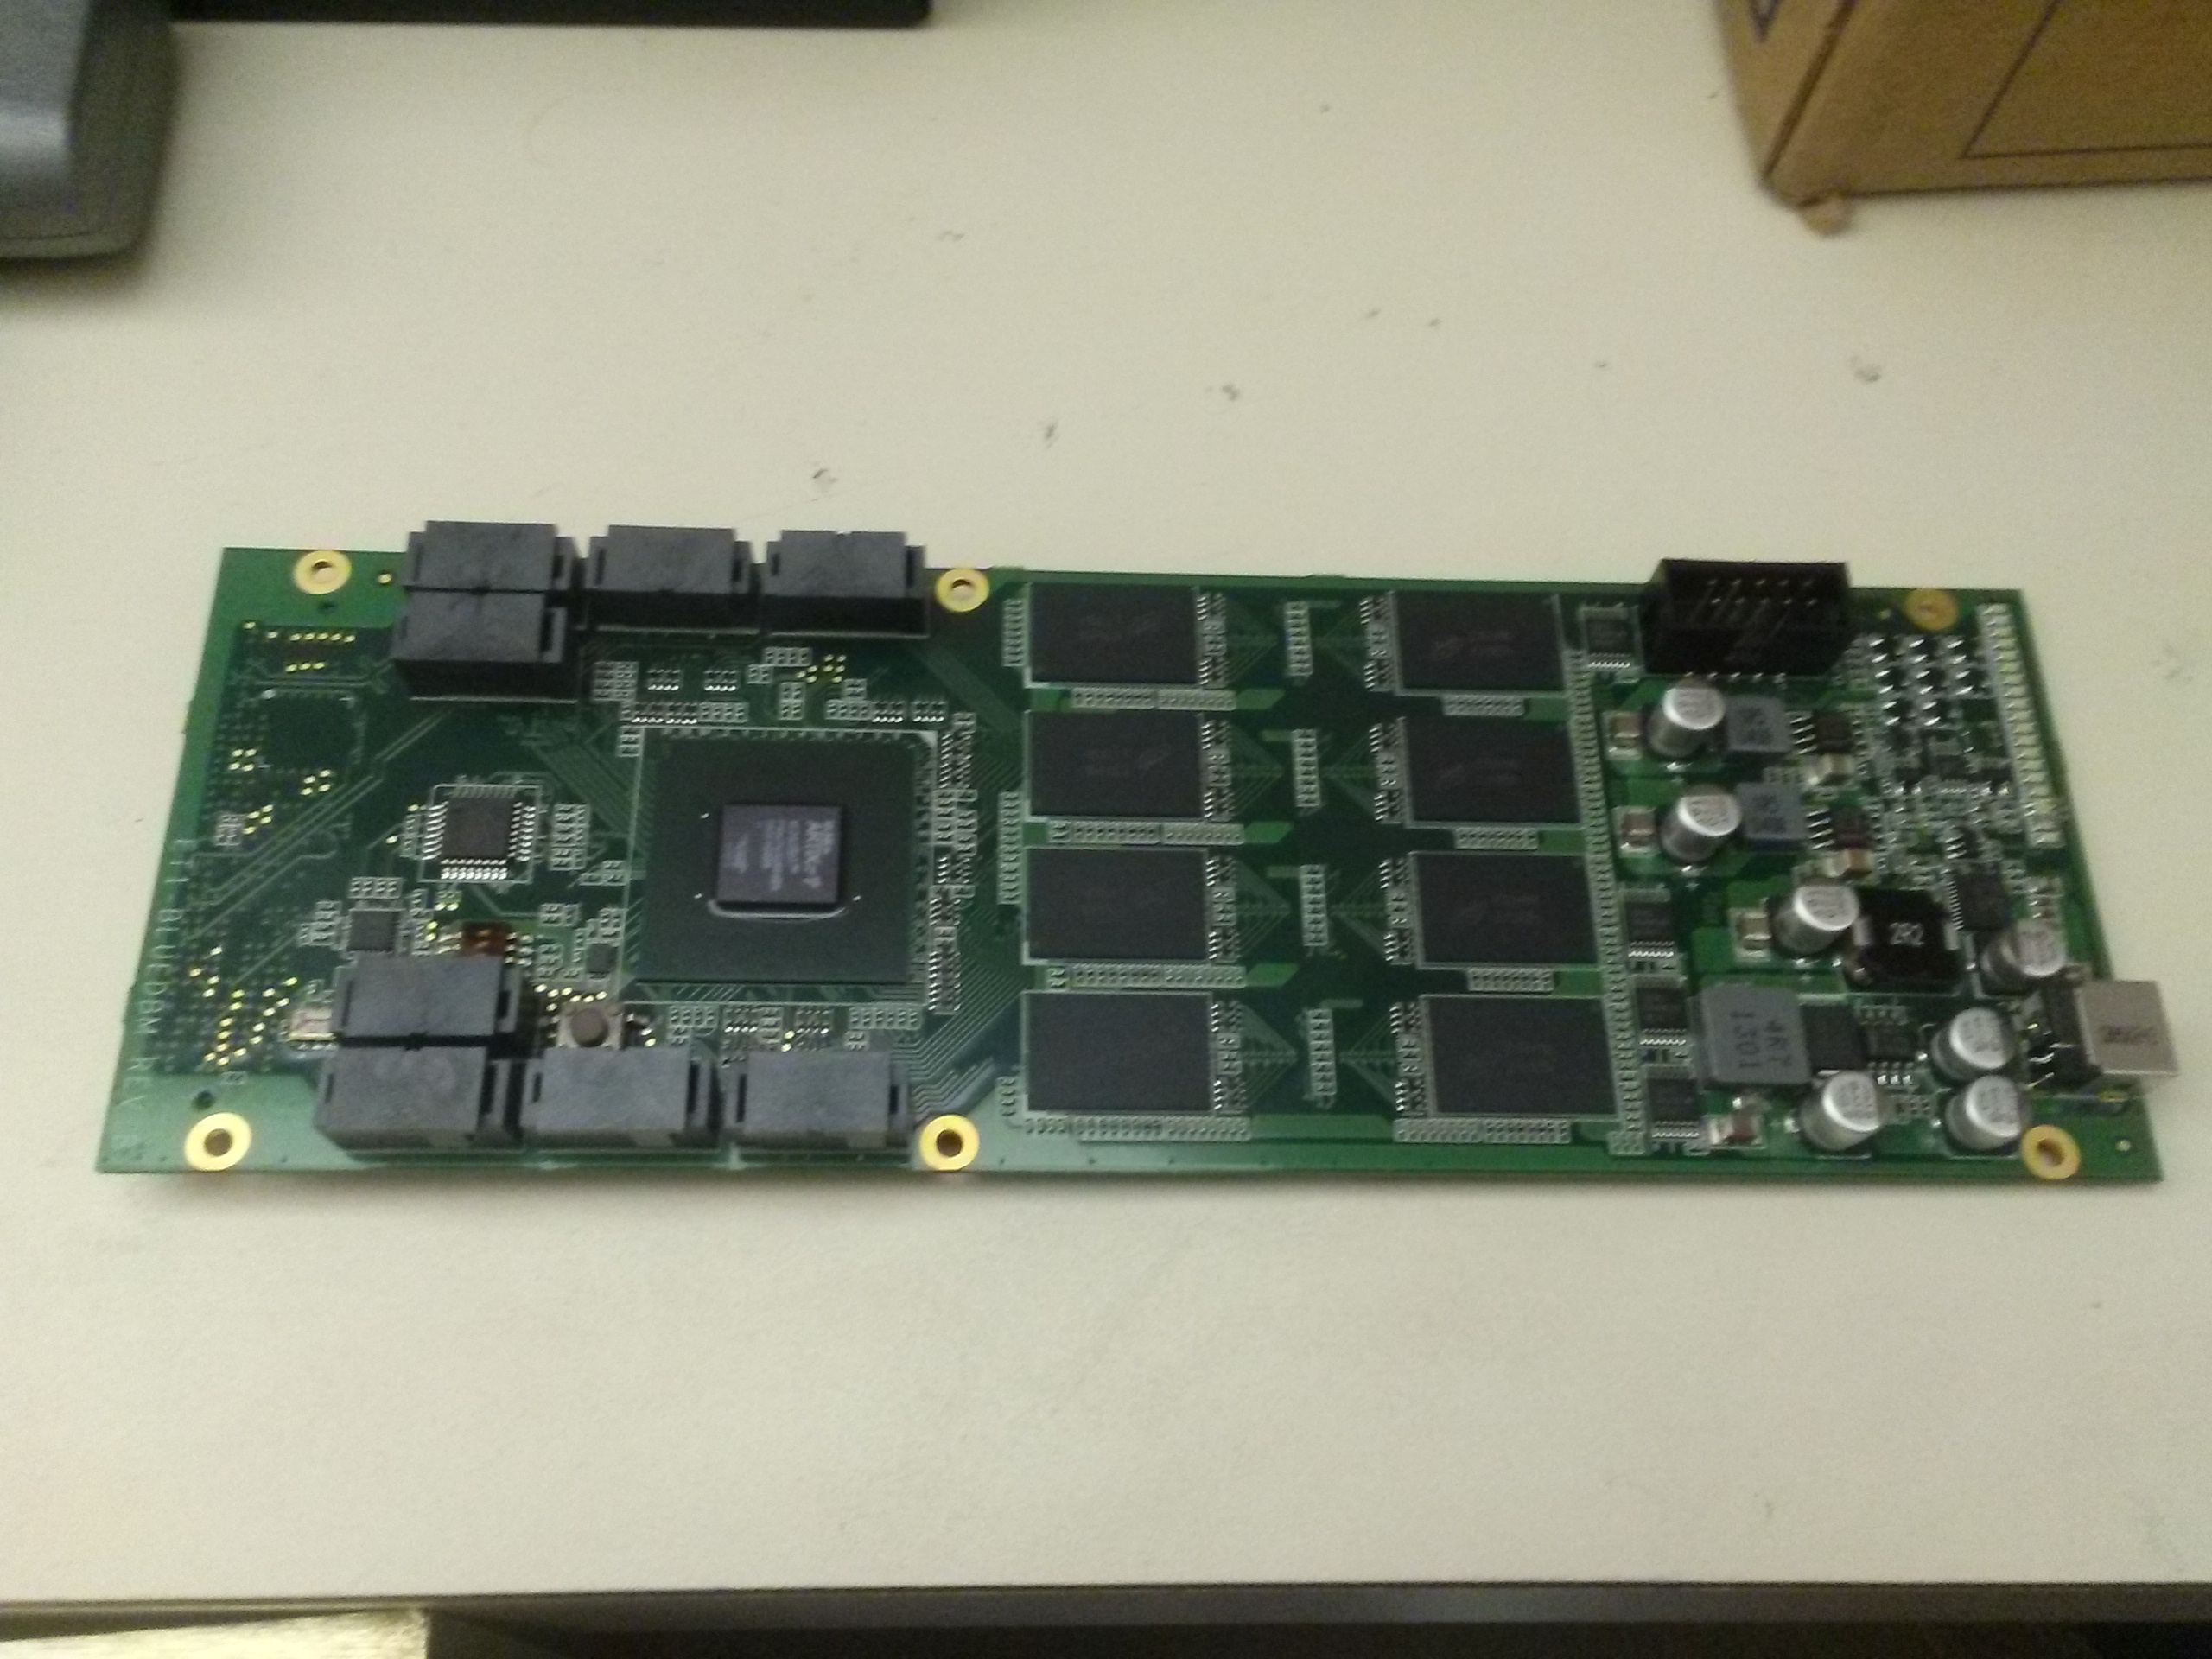
\includegraphics[width=\textwidth]{figures/flashboard.jpg}
	\caption{A Custom Flash Card}
	\label{fig:flashboard}
	\end{minipage} \\
	&
	\begin{minipage}[c]{.20\textwidth}
	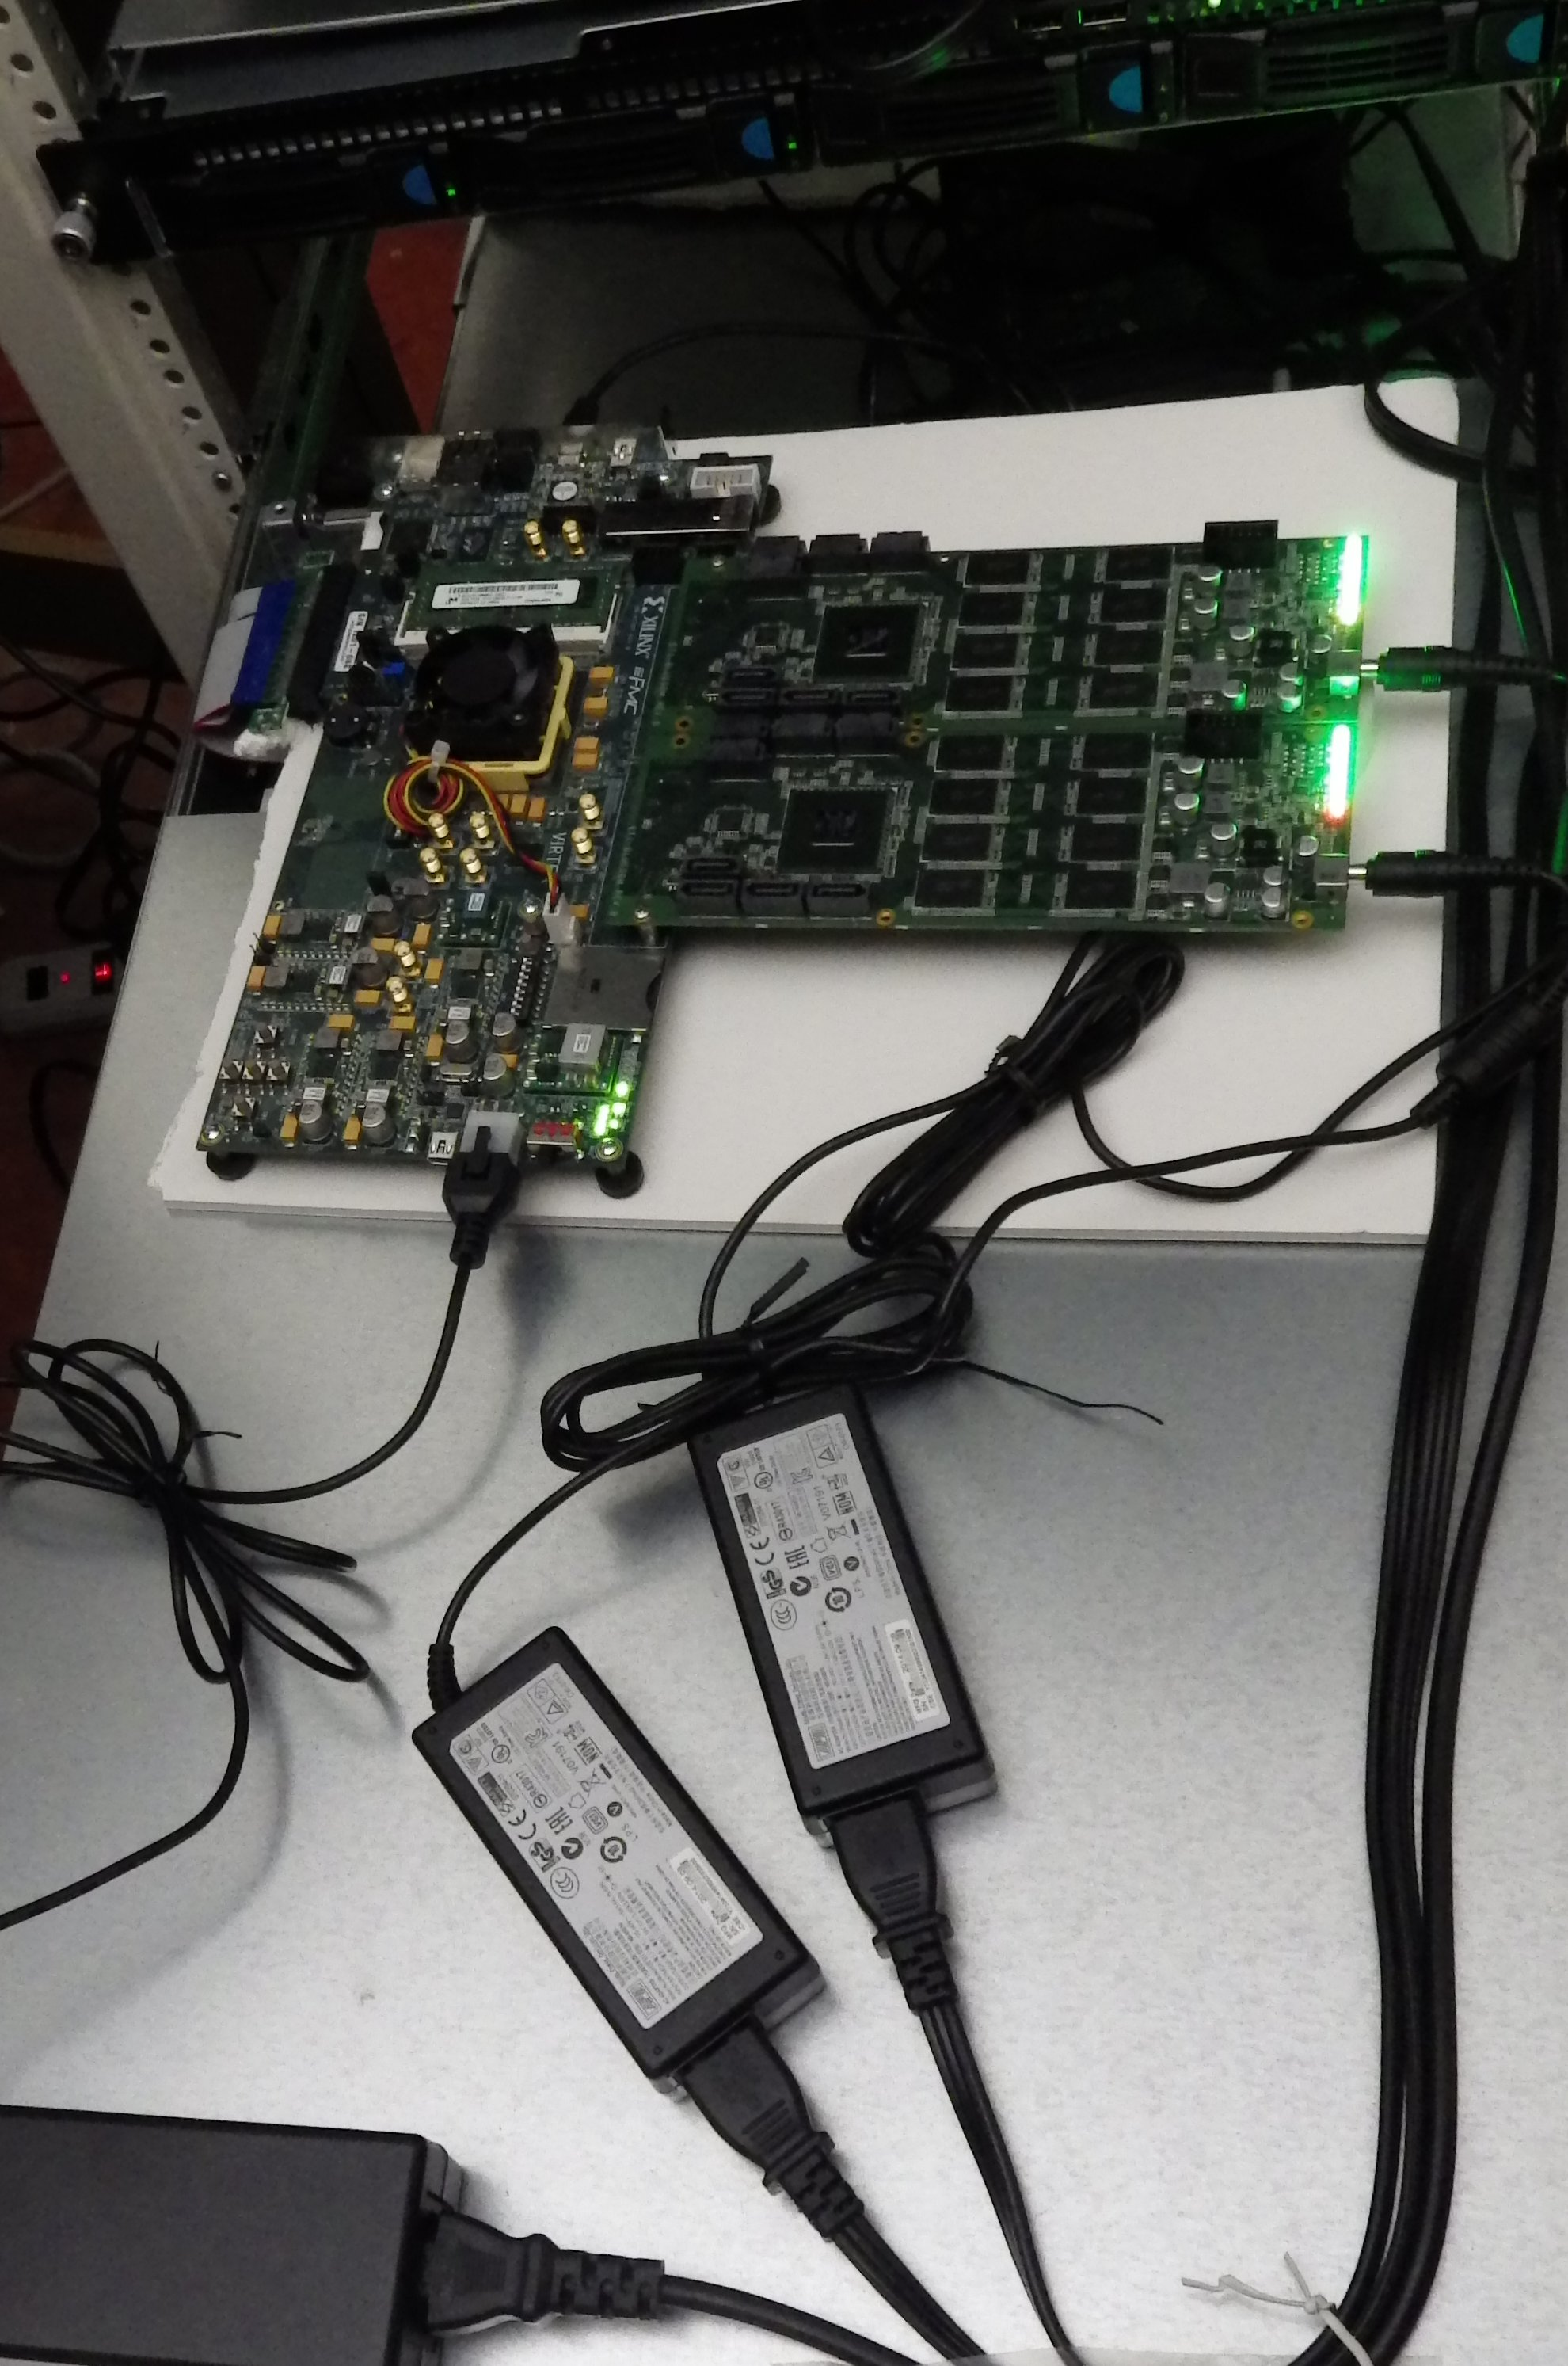
\includegraphics[width=\textwidth]{figures/racknode.jpg}
	\caption{A FlashBoost Rack Node}
	\label{fig:flashrack}
	\end{minipage}
	\end{tabular}
\end{figure}
%\begin{figure}[ht]
%	\begin{center}
%	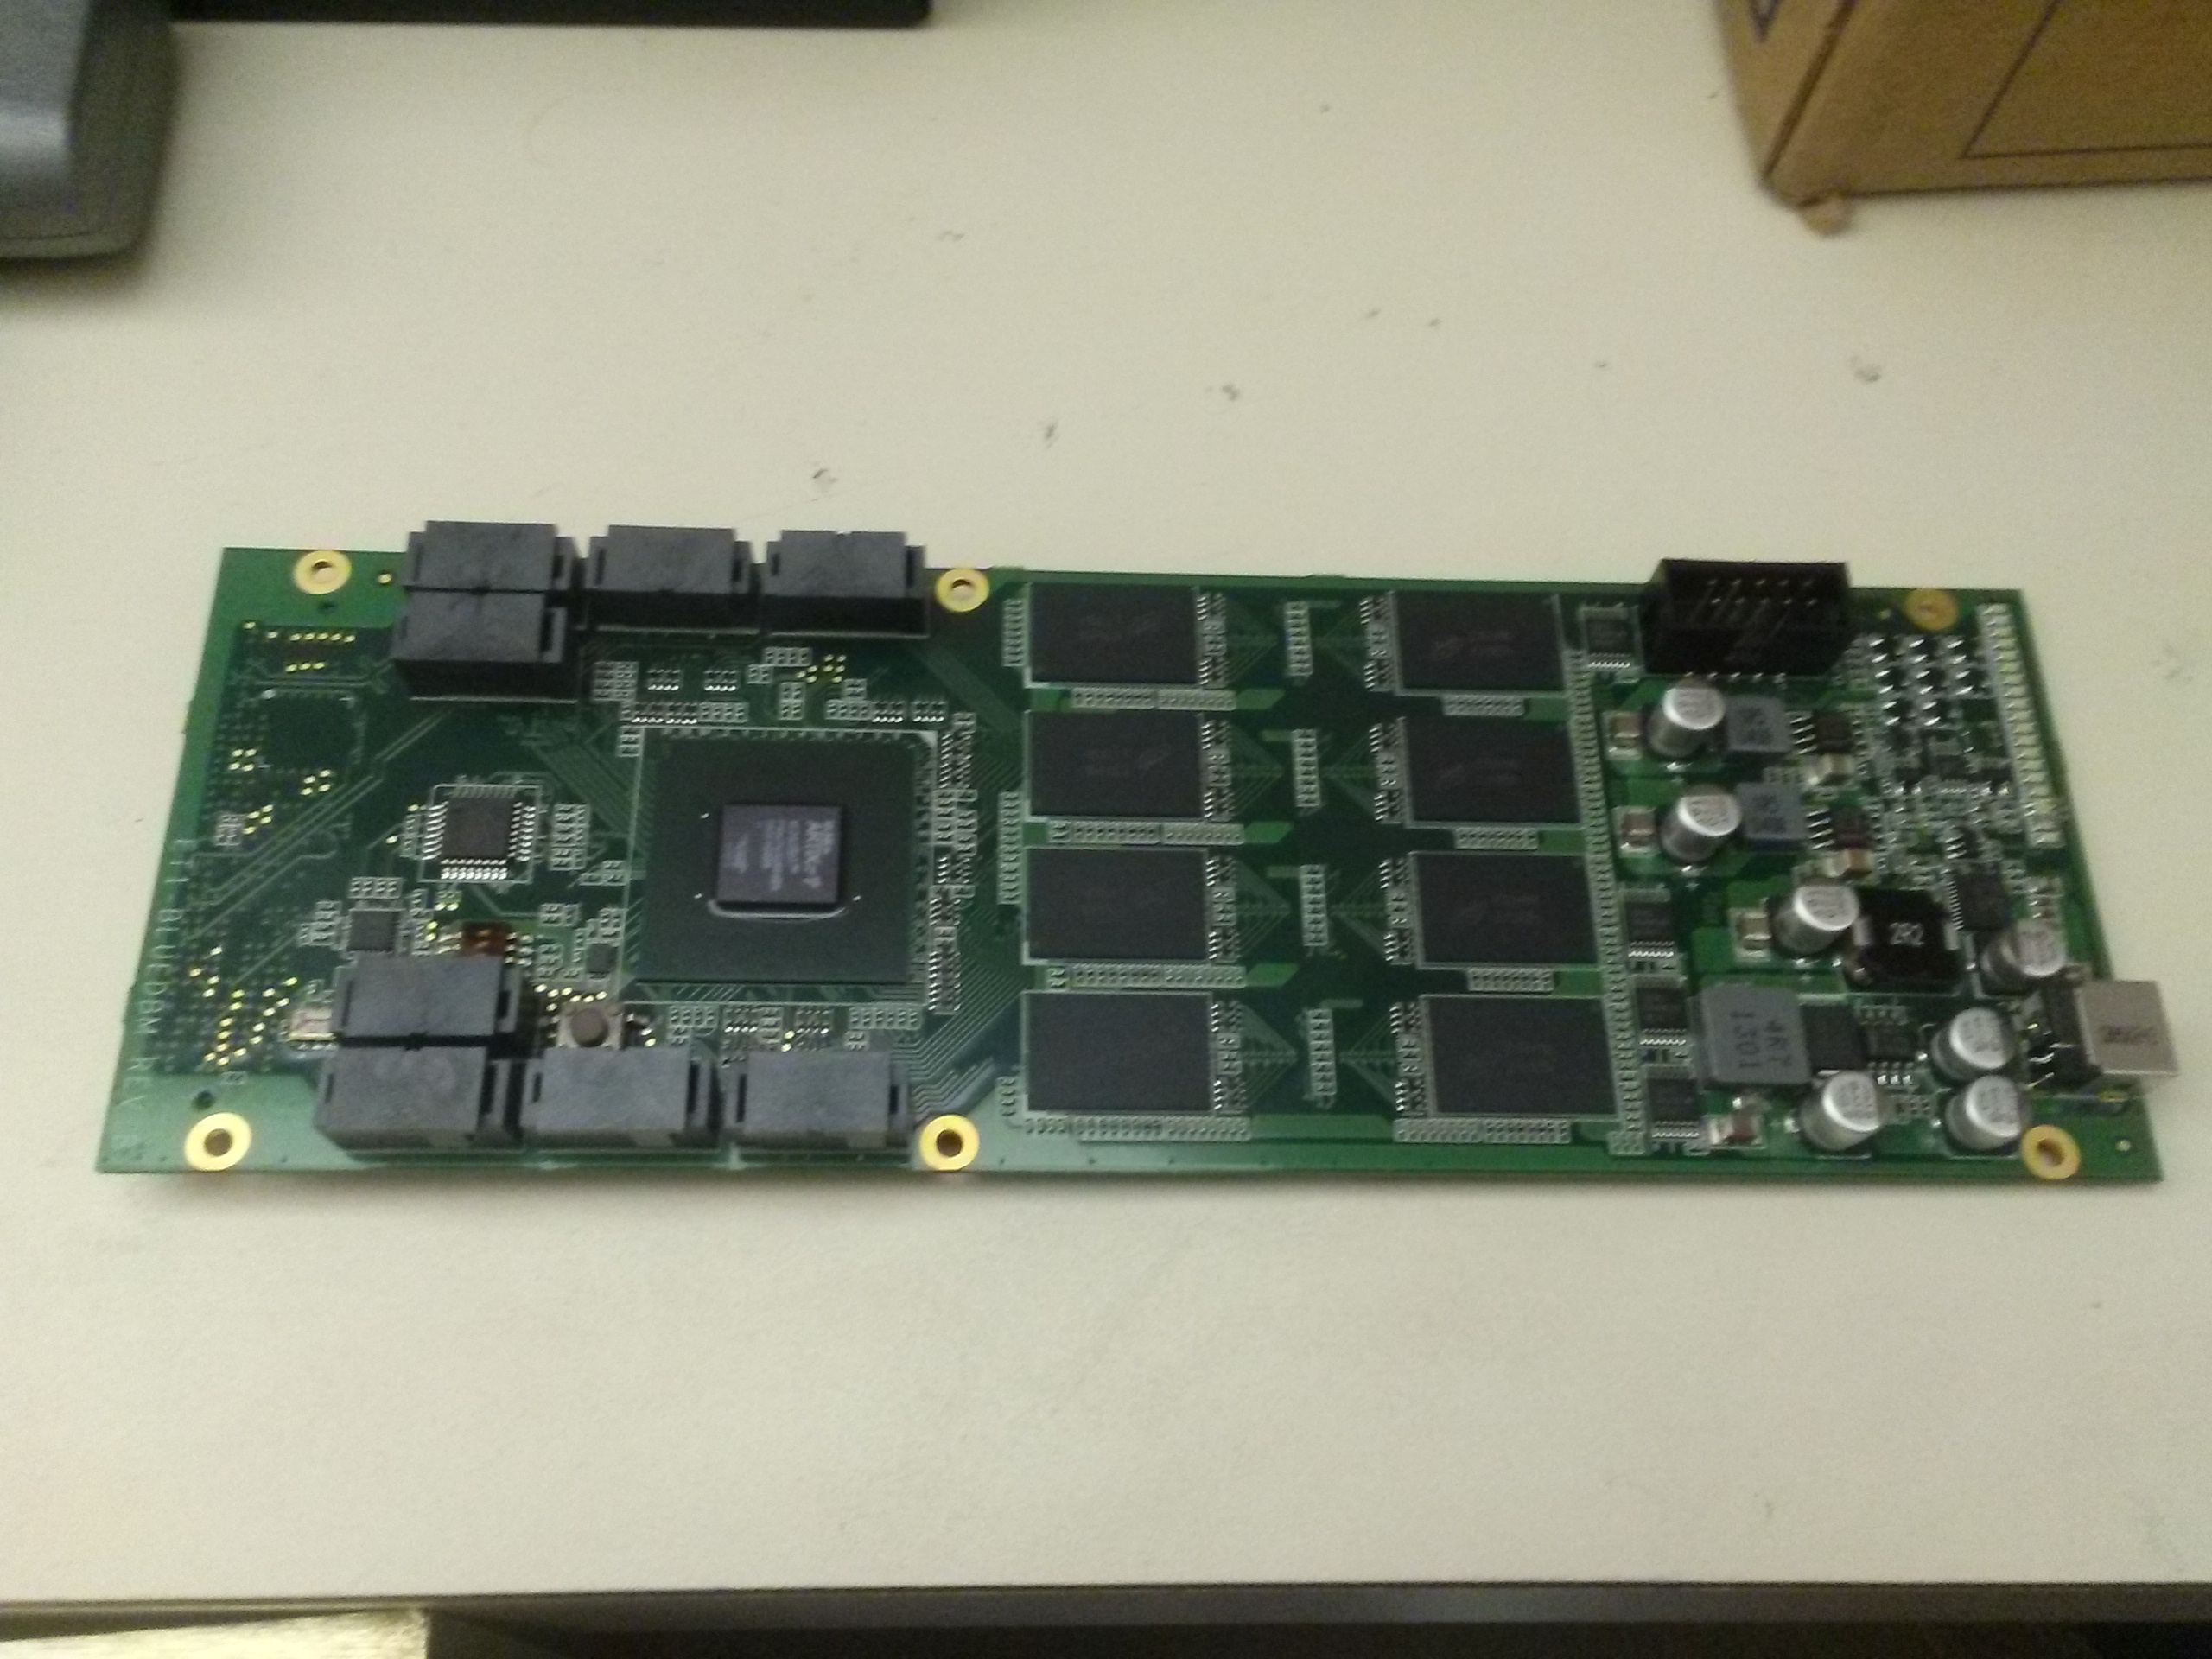
\includegraphics[width=0.4\textwidth]{figures/flashboard.jpg}
%	\caption{A Custom-Built Flash Board with 512GB of NAND Flash}
%	\label{fig:flashboard}
%	\end{center}
%\end{figure}
%	\subfloat[One of the two 10-node FlashBoost Racks]
%		{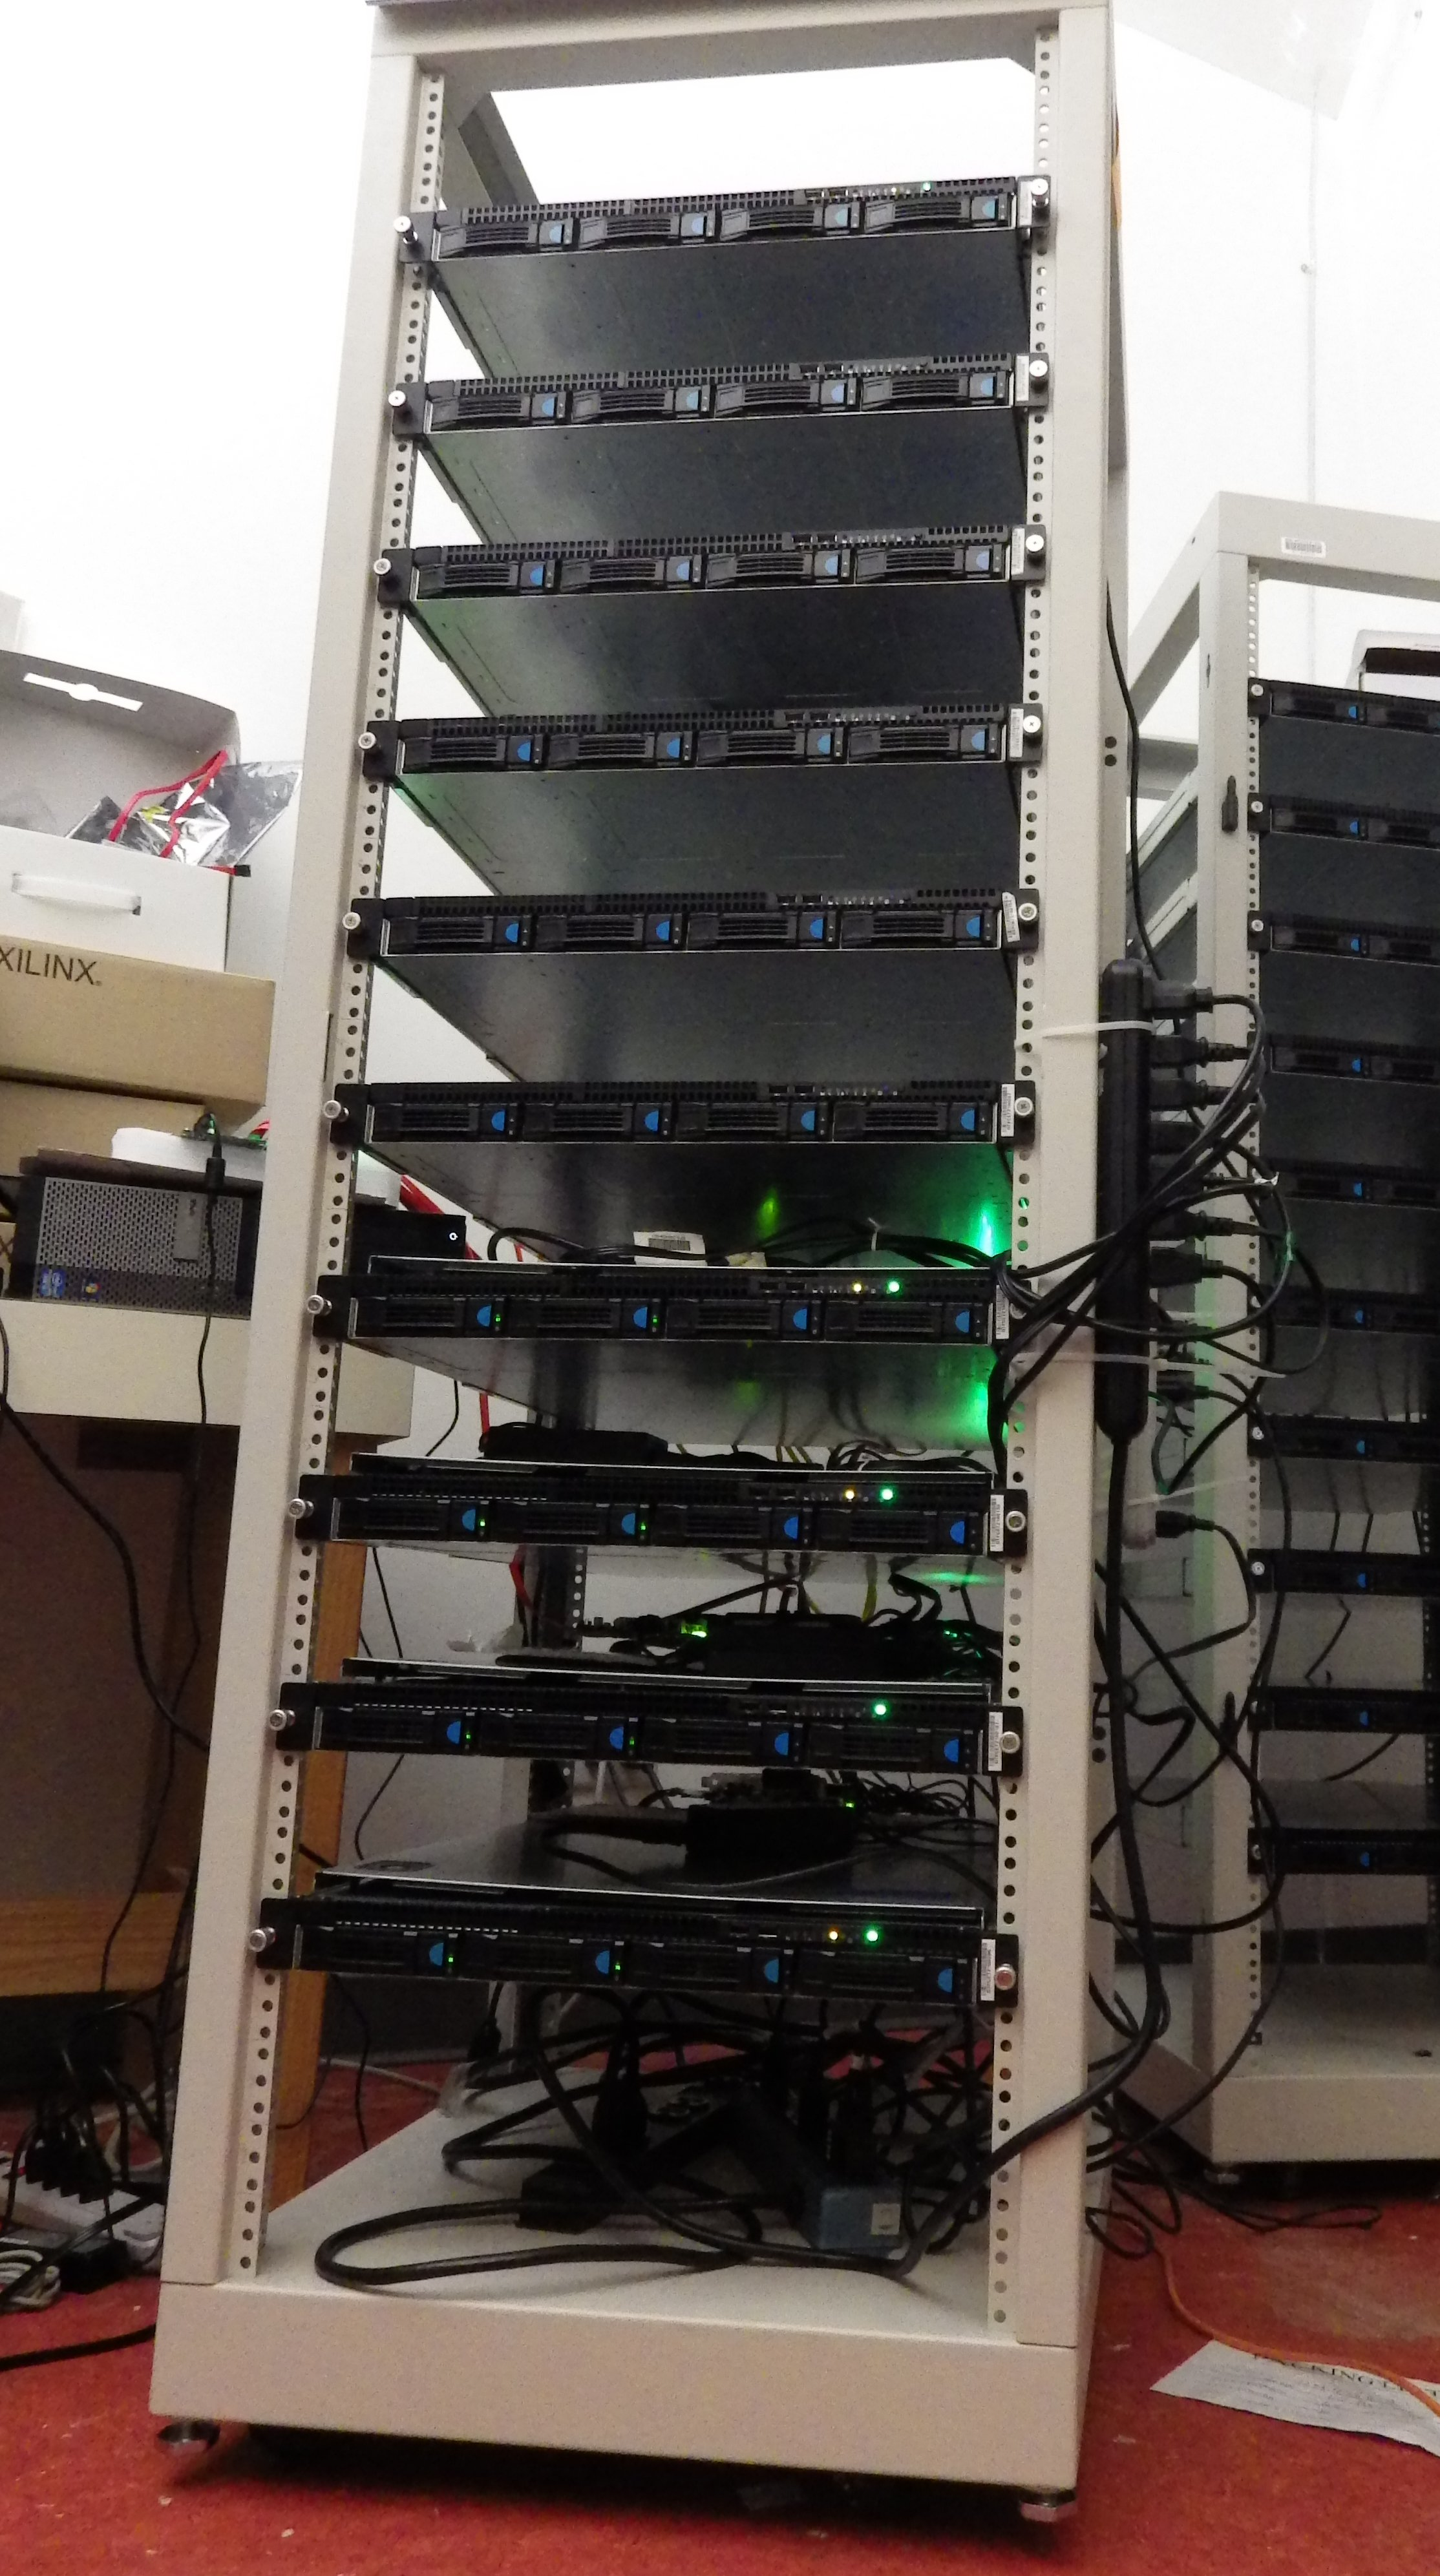
\includegraphics[width=0.22\textwidth]{figures/rackserver2.jpg}}
%	} 

In our implementation of FlashBoost, we have used a Field Programmable Gate
Array (FPGA) to implement the in-store processor and also the flash, host and
network controllers. However, the FlashBoost Architecture should not be limited
to an FPGA-based implementation.  Development of FlashBoost was done in the
high-level hardware description language Bluespec. As a result, all services
expose a high-level language interface using latency-insensitive FIFOs for
communication. This makes the services intuitive to use, and flexible to be used
easily with many in-storage processing engines.

The cluster consists of 20 Xeon servers mounted in two racks, each with a Xilinx
VC707 FPGA development board connected via a PCIe connection. Each VC707 board
hosts two custom-built flash boards with SATA connectors. The VC707 board,
coupled with two custom flash boards is mounted on top of each server.
The host servers run the Ubuntu distribution of Linux.
Figure~\ref{fig:bluedbmnode} shows the components of a single node.
One of the servers also had a 512GB Samsung M.2 PCIe SSD for performance
comparisons.

We used Connectal~\cite{connectal} and its PCIe Gen 1 implementation for the
host link. This PCIe implementation caps our performance at 1.6GB/s reads and
1GB/s writes, which is a reasonable performance for a commodity flash storage
device. In the future we will also explore the benefits of a faster host link
including later generation PCIe links.

\begin{figure}[ht]
	\begin{center}
	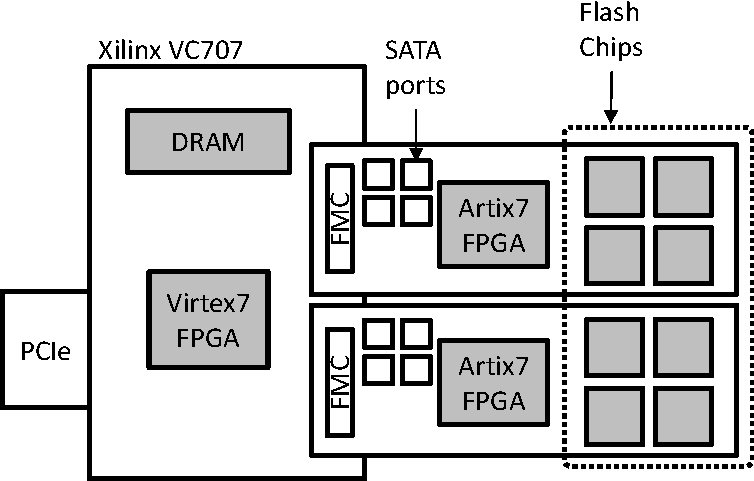
\includegraphics[width=0.3\textwidth]{figures/storagenode-crop.pdf}
	\caption{A FlashBoost Storage Node}
	\label{fig:bluedbmnode}
	\end{center}
\end{figure}


\subsection{Custom Flash Board}

%\begin{figure}[ht]
%	\begin{center}
%	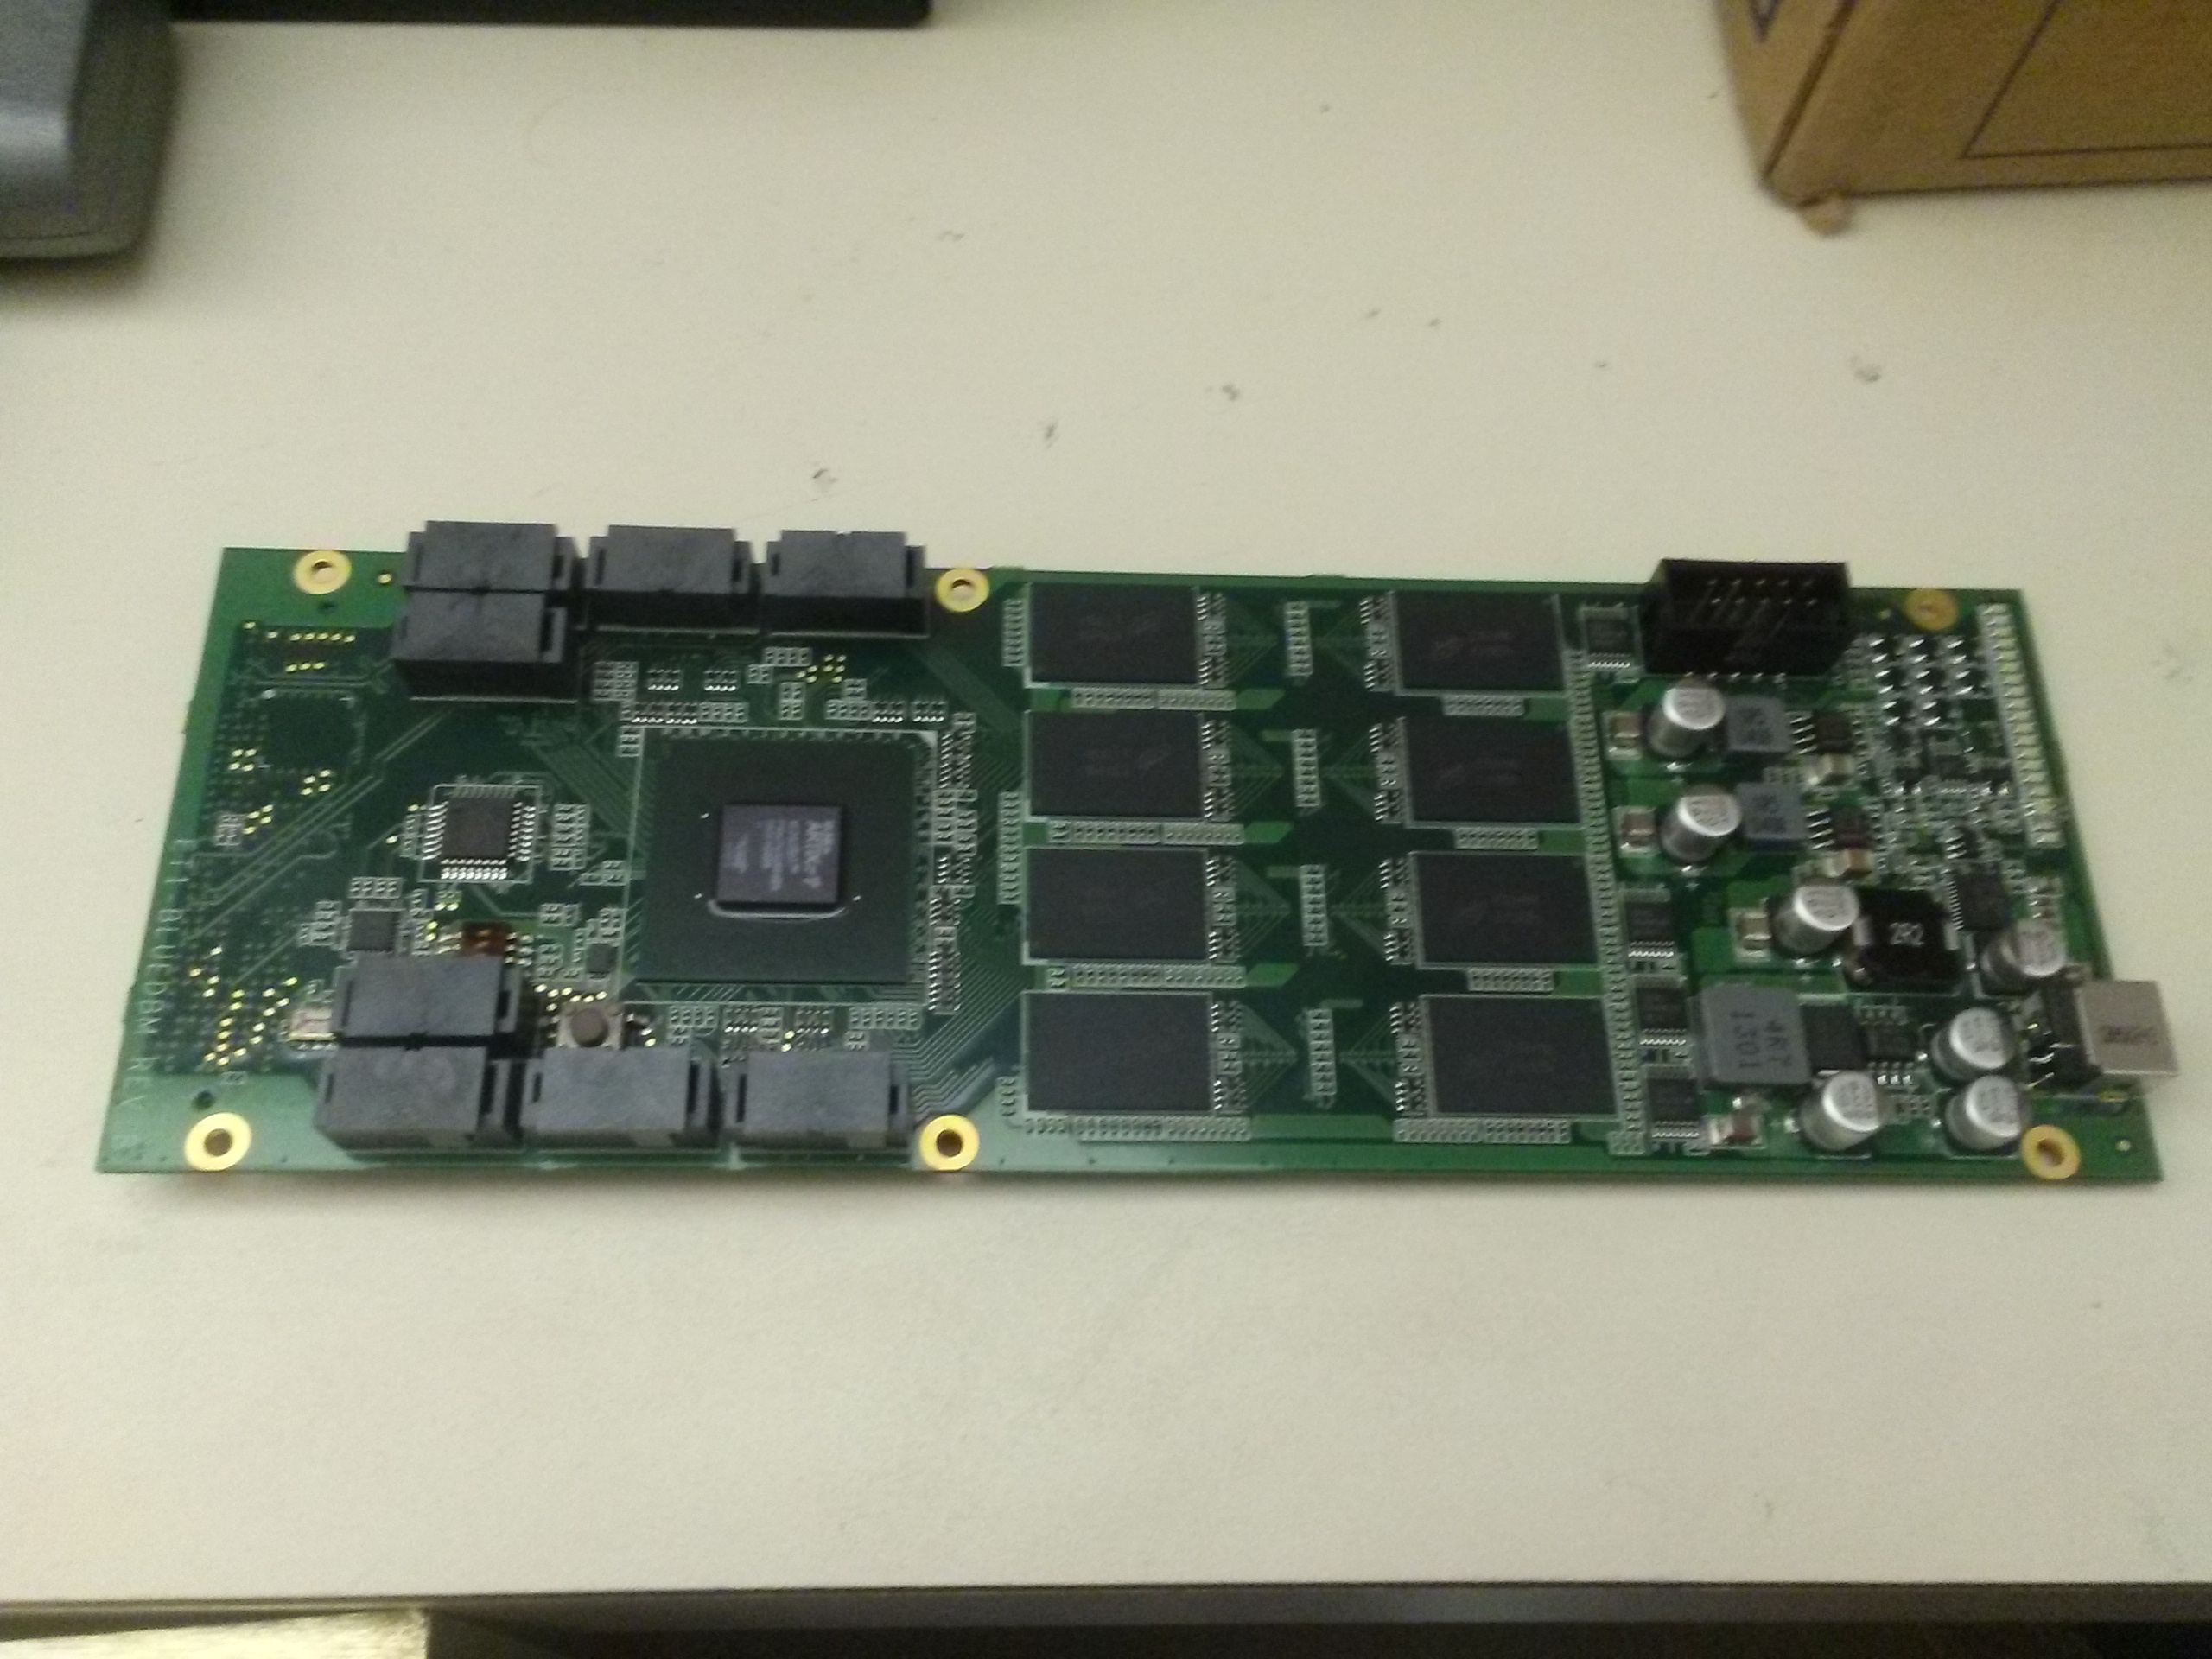
\includegraphics[width=0.4\textwidth]{figures/flashboard.jpg}
%	\caption{A Custom-Built Flash Board with 512GB of NAND Flash}
%	\label{fig:flashboard}
%	\end{center}
%\end{figure}

We have designed and built a high-capacity custom flash board with high-speed
serial connectors, with the help of Quanta Inc., and Xilinx Inc.

Each flash card has 512GBs of NAND flash storage and a Xilinx Artix 7 chip, and
plugs into the host FPGA development board via the FPGA Mezzanine Card (FMC)
connector. The flash controller and Error Correcting Code (ECC) is implemented
on this Artix chip, providing the Virtex 7 FPGA chip on the VC707 a logical
error-free access into flash. The communication between the flash board and the
Virtex 7 FPGA is done by a 4-lane aurora channel, which is implemented on the
GTX/GTP serial transceivers included in each FPGA. This channel can sustain up
to 3.3GB/s of bandwidth at 0.5$\mu s$ latency.
The flash board also hosts 8 SATA connectors, 4 of
which pin out the high-speed serial ports on the host Virtex 7 FPGA,
and 4 of whch pin out the high-speed serial ports on the Artix 7 chip.
The serial ports are capable of 10Gbps and 6.6Gbps of bandwidth, respectively.

\subsection{Network Infrastructure}

In our FlashBoost implementation, the link is implemented over the
low-latency serial transceivers.  By
implementing routing in the hardware and using a very low-latency network
fabric, we were able to achieve very high performance, with less than 0.5$\mu s$ of
latency per network hop, and near 10Gbps of bandwidth per link. Our
implementation has a network fan-out of 8 ports per storage node, so the
aggregate network bandwidth available to a node reaches up to 8GB/s, including
packet overhead.

\subsection{Software Interface}

Our host interface was implemented using Connectal~\cite{connectal}, a
hardware-software codesign framework built by Quanta Research Cambridge.
Connectal reads the interface definition file written by the programmer and
generates glue logic between hardware and software. Connectal automatically
generates RPC-like interface from developer-provided interface specification, as
well as a memory-mapped DMA interface for high bandwidth data transfer.
Connectal provides a PCIe Gen 1 endpoint and driver pair, and provides up to
1.6GB/s DMA read to host DRAM bandwidth and 1GB/s of DMA write from host DRAM
bandwidth. 

Reading or writing data from the host buffers were done by DMA read/write
engines implemented in the Connectal framework. In our FlashBoost
implementation, there are four read engines and four write engines each, in
order to more easily make maximum use of the PCIe bandwidth. 



\section{Results}
\subsection{Configurations}

\subsection{Distributed Flash Access Performance}
Latency for local flash reads, reads from local DRAM, remote reads over
fpga/serial, remote reads over serial/host DRAM, remote reads over
ethernet/Flash ethernet/DRAM

Aggregate bandwidth for flash, collecting all flash to one node, flash to pcie?

Aggregate bandwidth for competing workloads on multiple servers \(scalability\)

\subsection{Distributed Analytics Performance}

Measure latency of 8K page reads + filtering for flash, host DRAM, remote flash,
remote host DRAM, remote host DRAM with sw filtering


\section{Application Acceleration}
\label{sec:acceleration}

In this section, we demonstrate the performance and benefits of the FlashBoost
architecture by presenting some simple accelerator examples. 

\subsection{Nearest Neighbor Search}

Nearest neighbor search is a classical problem with many applications. One of
the modern achievements in this field is Locality Sensitive Hashing~\cite{lsh}.
LSH hashes the dataset using multiple hash functions, so that
similar data is statistically likely to be hashed to similar buckets. When
querying, the query is hashed using the same hash functions, and only the data
in the matching buckets are actually compared. The bulk of the work during a
query process is traversing hash buckets and reading the corresponding data to
perform distance calculation. Because data pointed to by the hash buckets are
most likely scattered across the dataset, access patterns are quite random.

We have built a LSH query accelerator, where all of the data is stored in flash
and the distance calculation is done by the in-storage processor on the storage
device. For simplicity, we assume 8KB data items, and calculate the hamming
distance between the query data and each of the items in the has bucket. The
software sends a stream of addresses from a hash bucket along with the query
data, and the system will return the index of the item most closely matching the
query. By offloading computation to the in-storage accelerator, we
show XXX\% performance improvement over the non-accelerated implementation.



\subsection{Graph Traversal}

Efficient graph traversal is a very important component of any graph processing
system. It is also a very latency-bound problem because one often cannot predict
the next node to visit, until the previous node is visited and processed. We
demonstrate the performance benefits of our FlashBoost architecture by
implementing graph traversal that takes advantages of the in-storage processor
and the integrated storage network, which allows extremely low-latency access
into both local and remote flash storage. The difference latency has on graph
traversal queries can be seen in Figure~\ref{fig:graph_accel}. We demonstrate that compared to a
naive implementation that uses flash only as a storage device, we have XXX\%
performance improvement.

%\begin{figure}[h]
%	\begin{center}
%	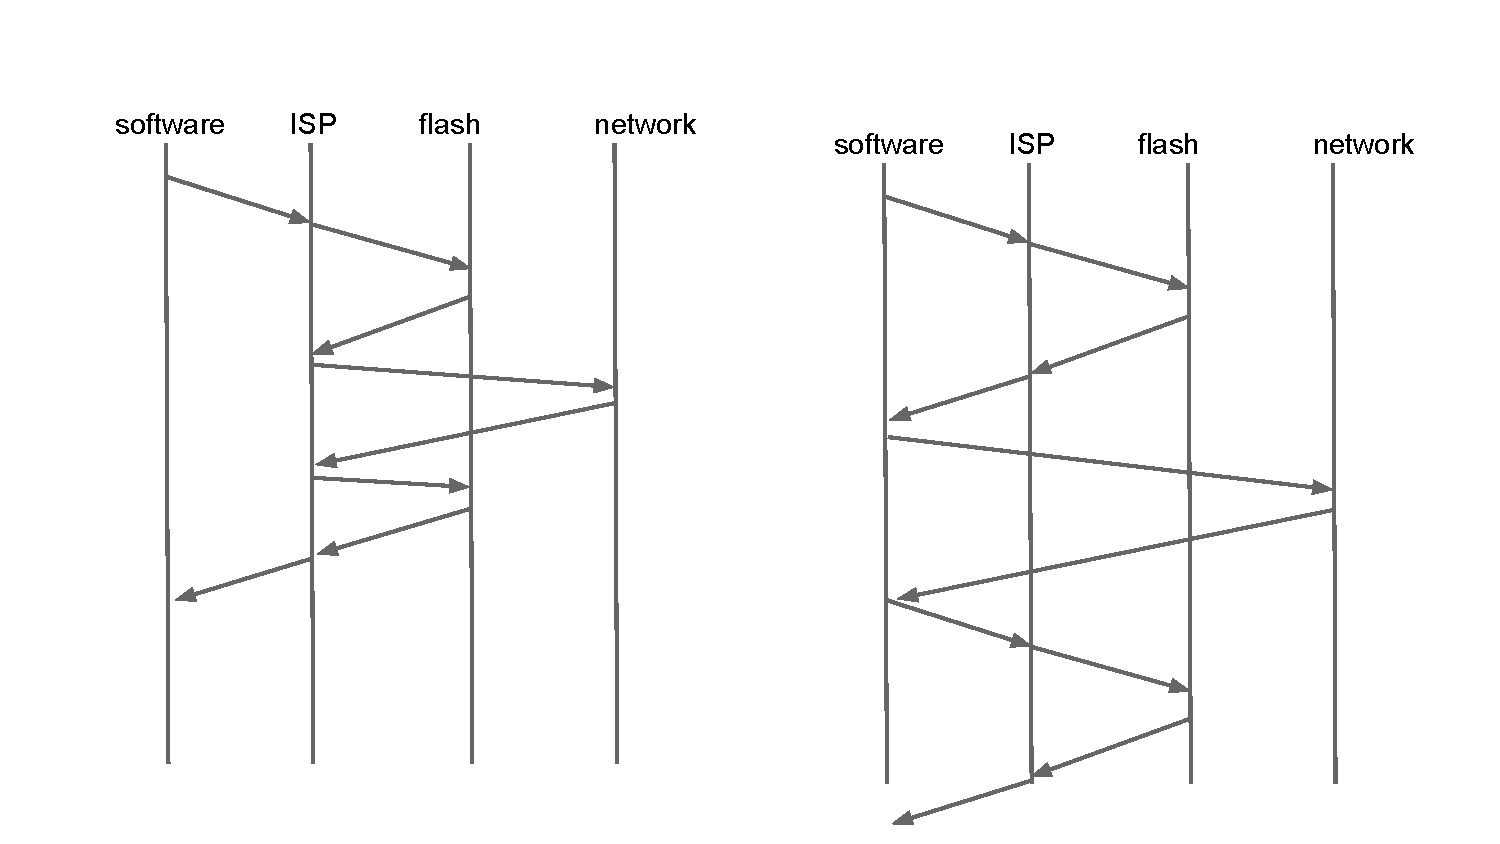
\includegraphics[width=0.4\paperwidth]{figures/graph_accel.pdf}
%	\caption{Graph Traversal Comparison}
%	\label{fig:graph_accel}
%	\end{center}
%\end{figure}

\begin{figure}[ht!]
	\centering
	\subfloat[Using ISP and Integrated Network]
		{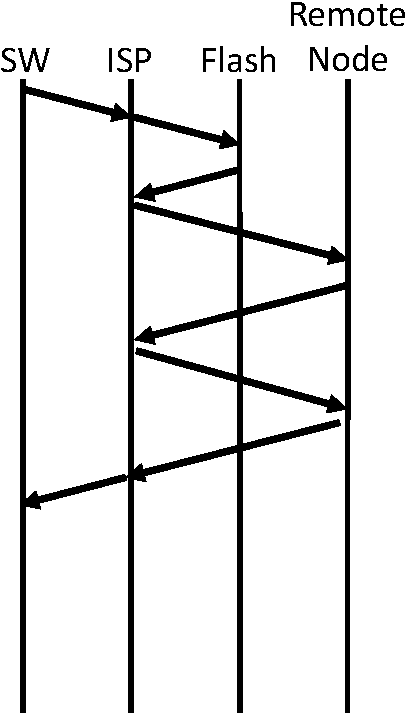
\includegraphics[width=0.18\textwidth]{figures/graph_isp-crop.pdf}}
		\hfill
	\subfloat[Using Software]
		{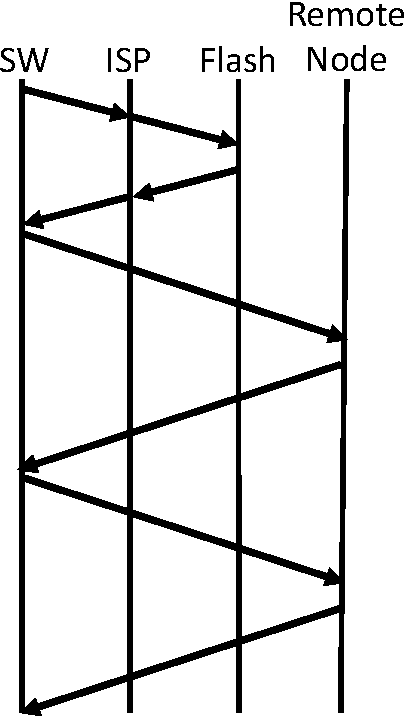
\includegraphics[width=0.18\textwidth]{figures/graph_sw-crop.pdf}}
		\hfill
	\caption{Graph Traversal Comparison}
	\label{fig:graph_accel}
\end{figure}

\subsection{String Search}

String search is common operation in analytics, often used in
database table scans, DNA sequence matching and cheminformatics. It is 
primarily a sequential read and compare workload. We
examine its performance on FlashBoost with assistance from in-store Morris-Pratt (MP) 
string search engines~\cite{?} fully integrated with the file system, flash controller
and application software.  The software portion of string search initially sets
up the accelerator by transferring the target string pattern (needle) and a set
of precomputed MP constants over DMA. Then it consults the file system for a
list of physical addresses of the files to search (haystack).  This list is
streamed to the accelerator, which uses these addresses to request for pages
from the flash controller.  The accelerated MP engines may operate in parallel
either by searching multiple files or by dividing up the haystack into equal
segments (with some overlaps). This choice depends on the number of files and
size of each file. Since 4 read commands can saturate a single flash bus, we
use 4 engines per bus to maximize the flash bandwidth. Only
search results are returned to the server. 




\section{Conclusion}

\bstctlcite{bstctl:etal, bstctl:nodash, bstctl:simpurl}
\bibliographystyle{IEEEtranS}
\bibliography{references}

\end{document}

